\chapter{`Transmission belt' model results \label{chapter:connectedModels}} 

\section{Introduction}

This chapter presents a model of the `transmission belt' between production and consumers able to produce equilibrium outcomes. These are `general' in the sense that they link supply and demand. It developed through the logical journey of building the model framework, with the models presented in chapter \ref{chapter:models} representing some of the important stepping stones revealing which choices could possibly work and which were less promising. 

The chapter is organised as follows:

\begin{itemize}
	\item Section \ref{sec:partialtogeneral} discusses elements that were rejected as possible routes to creating a `general' model capable of fully linking supply and demand in a completely open geography where agents were able to make decisions separately.
	\item Section \ref{sec:prodtowelfare} introduces the structure of the transmission belt model. The following sub-sections develop each stage of the transmission belt model systematically, looking at the following: the stock target mechanism used by Firms to achieve an `efficient' production level; Firms' scope for using `markup' as a profit mechanism and the problems with implementing this fully into a competition dynamic; a non-spatial explanation of the model's key ability to transition between two different production `regimes', with one Firm emerging as a more-efficient producer.
	\item Section \ref{sec:TM_space} introduces distance into the transmission belt model. This is done initially with a two region model before examining the dynamic as more agents are added onto a continuous line. This section ends by combining the transmission belt model with the density cost approach, in order to illustrate a way in which the production regime transition can determine spatial morphology.
	\item The chapter ends with a brief summary; much of the analysis of the transmission belt model takes place in chapter \ref{chapter:conc}. For example, while comparisons to \gls{ge} are discussed throughout the chapter, there is a direct comparison to the \gls{coremodel} made in section \ref{cmcomp}.
\end{itemize}


\section{Moving from `partial' to `general' \label{sec:partialtogeneral}}

Producing partial models is a relatively straightforward task compared to getting agents to fully coordinate economic activity. Of the various approaches attempted within this research, many were not able to recreate stable outcomes. Here are two quick examples. One: if the goal is to connect People's labour to production, and thus to stock levels, but also to let Firms set good and wage prices, it is very difficult to get sensible stock levels. This chapter presents a model that solves this stock problem, but it does it by avoiding the \gls{dmr} problems identified in section \ref{sec:mobFirms}. Firms using price-setting behaviour have a hard time producing stable economic outcomes: stock tends either to crash to zero or to increase indefinitely, without prices finding an efficient stock level. It is also difficult to find any compromise position between partial and general models. For instance, Firms can be given unlimited stock to attempt to avoid the stock problems just discussed. 

Second, the problem of price signalling is thorny. The simple random money flow model in section \ref{sec:comm_costs} demonstrated a key part of the problem: treating money literally as a rivalrous good hits up against the tendency for the flow among many agents to `random walk' into an uneven distribution. The model result even with agents making more sophisticated maximising choices is that some Firms can end up with the entire money supply - more than they need - while others find themselves in the catch-22 of not being able to pay the wages to produce stock to sell to get money to pay wages. Any economic agent model faces being stuck between this na\”{\i}ve approach to money and finding some other method capable of signalling between agents. 

The approach of this chapter is to cut out one layer of complexity by making People exchange `input' (their time) for productive output directly, where the price for the latter is the former. This avoids the need for an intermediary to signal price. This builds on the idea from section \ref{sec:results} that the important spatial economic distinction is between the spatial and non-spatial component of the costs People face, not whether they are goods-based or wage-based. 

The conclusion goes into more comparative detail about the whole set of dependencies in the thesis model framework and puts them in the context of the role of assumptions in model building.

\section{The `transmission belt' between production and welfare \label{sec:prodtowelfare}}

%The features that distinguish the model are the result of the particular path the logical journey of model development has taken. It is as much the result of concepts that did not work as concepts that succeeded. It is \emph{one} way to thread a needle through the many dependency problems the thesis has discussed. As the conclusion discusses in more detail, there are likely many other ways of making these dependencies function effectively together to produce other agent-based spatial equilibrium models. 
This section presents a model that connects supply and demand resulting in stable equilibria. Production with economies of scale are linked to consumers' welfare. It builds on concepts developed in the preceding analysis, finding a solution that allows efficiencies from economies of scale to feed through to improvements in utility. The key features of the model are:

\begin{itemize}
\item People get goods directly as their wage. They buy goods directly with their time (a flow of `one day per day') which then enters into Firms' production functions. Goods are sold using the `goods plus distance cost' equation from section \ref{sec:costmovinggoods}, $P_g = p_g + (c \cdot d)$. Goods and wage decisions are thus combined into a single utility decision.
\item Firms charge base price $p_g$ (the cost in a Person's time to buy one unit of good). Goods are exchanged directly for People's time, which then goes directly into the production function. Any good-movement costs `melt away'.
\item Production has economies of scale: higher input produces a higher per-unit output. A `smooth' \gls{eos} function is used where any increase in input translates into a higher-ratio output; no fixed labour component is required (section \ref{sec:prodfuncts}). 
	\item Economies of scale work as described in section \ref{sec:abmprod}: each Person `leaves' their time with each Firm they contribute to until their next decision point. The production of stock is based on the amount of contributed time at each decision point.
\item People use a \gls{ces} function to buy goods and distribute their time to Firms. This circumvents \gls{bertcomp}-like problems with wage-setting, where a wage offer only minutely higher than others will automatically be selected. It means that each Person buys at least a little from each Firm - and thus contributes time to each - unless $\rho = 1$, in which case goods are fully substitutable and the cheapest will be bought.
	\item Demand for goods is always met: from the point of view of consumers, there are no stock limitations. The key advantage of this for the model is that a constrained utility function can be used safely: a consumer buys a given amount based on the set of prices they observe. They face no risk of stock running out.
	\item Firms must then make sure that stock levels keep close to the amount being produced (or more than this amount if they are seeking to make a profit; see below). They do this by setting good costs to target a stock level - net zero stock if they are not attempting to skim a profit.
\end{itemize}

In contrast to the two-timestep feedback decisions of Firms (used in section \ref{sec:mobFirms}) stock levels are controlled through ongoing `granular' price adjustments. These are, as Leijonhufvud puts it, `laws of motion' (section \ref{sec:ace}) describing how Firms respond to changes in stock. This adjustment occurs every time a Person buys. It is a `market mechanism' in that price signals are used by Firms to optimise a particular quantity though, as section \ref{sec:markup} discusses, while prices are used and interact to produce the equilibrium outcome, Firms are not able to directly compete. The `granular' process that occurs each time a Person buys a good is as follows:

\begin{itemize}
\item A Person chooses their best Bundle as described in section \ref{sec:howPeopleAct} using their unit of time as the budget. Since it is a \gls{ces} function, all Firms will receive some share of this (see section \ref{sec:utilspace}) minus the distance cost that `melts away'; that is, any time a Person spends on distance does not enter into production.
\item When each Firm receives a signal that a Person is buying, it pays with the appropriate quantity of good based on its current price and stock is reduced accordingly. 
\item The quantity of input the Firm receives in return goes straight into production. The production amount is worked out as described in section \ref{sec:abmprod}: economies of scale come from all input from recent interactions, and the actual productive output is calculated when the Person buys. It is proportional to the time that Person contributes. The method of achieving this is to use the smooth \gls{eos} function described in section \ref{sec:prodfuncts}.
\item There is now a net stock level from this one interaction, which the Firm uses to guide their price adjustment. If stock is more than zero, demand is lower than production, and so the price is lowered to try and sell more. If stock is less than zero, demand was higher than production, and so the price is increased to sell less. 
\item The change in price is proportional to the amount that stock levels deviate from the target amount: $\triangle p_g = f(stock)/x$, where $x$ controls the magnitude of the price change. See section \ref{sec:stocktarget} for an explanation of the chosen function for stock targeting.
\end{itemize}

Stock can go below zero for a time; this is vital for the price signal to target it from both sides of the zero line, though the net stock target over time is ideally zero. This zero target can be made physically `plausible' by assuming Firms have stock buffers. Zero then becomes their target production level rather than a physical lower limit. Indeed, the model can be set up to reach a given arbitrary level of production and then work from there, leaving a positive buffer. For the sake of ease of discussion, though, a target of zero is assumed (except for section \ref{sec:markup} which uses the choice of stock target as a way for Firms to seek profit).

Secondly, in contrast to the `blind versus rational' problem described in section \ref{sec:blindvsrational}, the transmission belt model \emph{can} work with the fixed-cost, \gls{coremodel} style of production function - but only if total input is able to exceed the fixed labour requirement. Otherwise, People buy goods that the Firm then cannot possibly make, since the production function becomes negative. Because of the fact that People `leave' their time with Firms over an iteration, the fixed labour requirement can be met, but it leads to some nonsensical situations like the one just described. The smooth \gls{eos} function produces more reliable outcomes for the transmission belt model.

Lastly, a deeper explanation of the role of stock targeting in the model and its relation to efficiency (details of the actual mechanism are discussed below in section \ref{sec:stocktarget}). The motivation was to find a way of linking labour input to good output and consumption. This requires all goods to be priced correctly. Many of the coordination problems involved in doing this have been discussed, especially the issue of getting time input to feed through to more efficient good production via economies of scale (section \ref{sec:abmprod}). 

What does `efficient' mean in this context? A given amount of time input into a Firm equates to a given level of good output via its production equation. The most efficient level of production from the point of view of People is where net stock from \emph{all} Firms remains as close to zero as possible. Less than zero stock is both nonsensical in the long run and indicative that economies of scale are not being exploited as fully as they could be. Positive stock levels indicate that People are not getting all the available output that their labour is creating. The zero stock target is thus the point at which the benefits from production are maximised and feed through to utility levels.

This approach described above succeeds in finding efficient equilibria. In situations with many Firms and People, each Firm is able to find a unique price that keeps its own stock levels efficient while buying and selling to each Person. Their price signals find a balance point between production and People's utility demands as each Firms' price decisions interact with each other. (As explained below, the external effect of price changes are vital.)

%The `transmission belt' model can do some things the \gls{coremodel} cannot but, in doing so, is also (as it is presently constructed) unable to do others. It is able to find an efficient production equilibrium given the number of Firms set in the model. This \emph{does} succeed in linking efficient supply and demand through price signals. But it does not have a `market structure' in the sense of firms competing for custom. 
%\cmt{``But it does not have a `market structure' in the sense of firms competing for custom''. Yes it does! Kind of! This explanation needs a little more nuance so that it's clear price is linked to supply, demand, externalities.}
%This is an example where designing a model from the point of view of agents paid off. 
%In meeting the zero-stock target, the price signal must balance the two competing effects from changing the price. Reducing it increases demand, but it also increases input into production. That is not unique to this scenario: in any model with a small enough number of agents, changing price is always in effect changing the real wage. It must, however, find the point where these two balance. It cannot be described in the same way that a Firm would aim for $MC=MR$ (see section \ref{sec:marginalapx}) since the incoming and outgoings units are not the same. 
%Several interconnected problems need solving for this model to work. At the heart of the issue is cost, currency and stock. Implementing any kind of currency system is avoided by allowing the goods themselves to directly be the wage. This is made possible by using the \gls{ces} approach to getting inputs into production.
%Then, stock levels need to avoid two pitfalls. First, for economies of scale in production to feed through to welfare, any efficiency gains needed to actually be consumed. 
%The first solution is, as Fowler does (see section \ref{sec:fowler}), to always allow demand to be met. 
%The equilibrium reached by the transmission belt model is a full supply-demand equilibrium, but there is no way of knowing what a competitive equilibrium would look like in the core model sense.

\subsection{The stock targeting mechanism \label{sec:stocktarget}}

This section demonstrates how the transmission belt model and the stock target mechanism work. It compares two model runs with no distance cost: a `one Firm, one Person' model and another with fifty of each. A third model run adds a distance cost and randomly locates fifty of each agent type to illustrate the model's ability to equilibriate when agents face heterogenous costs imposed by location differences.

For the examples used in many of the following sections, the smooth \gls{eos} equation is kept in its normalised form of $t^2 + t$, with neither the curve or straight line parameter changing its scale. This allows for some useful simplifications that aid understanding of what the model is doing. 

In the case of only one Firm, and assuming there are no distance costs, there is a very straightforward deduction of the correct price for `clearing the market' and this can be compared with the model outcome. If there is only one Firm, all input goes into that single Firm: People have nowhere else to buy from and will spend everything they have there. So (assuming no space costs) the Firm's output is directly proportion to the number of People, since each Person contributes a single unit of input. A Firm wants to clear its stock - to keep it as close to zero as possible. What price can it set to do this? Price is the output a Firm gives for a unit of input. People pay with a unit of input each so, in this simple case, price is always just the number of people divided by total output. Using the smooth \gls{eos} function and setting both the curve and magnitude parameters to one, output is just $t^2 + t$ (where $t$ is the total input from all People). In cases where only one Person is contributing one unit of $t$ to each Firm, the price equation reduces to $P = 1/(t+1)$. In the case of one Firm and one Person, then, at equilibrium $P = 0.5$. 

In model runs with no distance cost, deducing the equilibrium price is straightforward for other mixes of Firm and Person number, as long as demand is either spread evenly or being input into a discrete subset of Firms, as happens when one Firm emerges as a selected site for large-scale efficient production (see section \ref{sec:lov_vs_eos} below). If demand is spread evenly, output and price is the same as above. If, for example, two hundred people input into fifty Firms evenly, that is four People's time per Firm. Equally, if one efficient producer emerges, all fifty People input their time into that Firm's smooth \gls{eos} equation.

As explained, in the transmission belt model, each Firm adjusts their price in order to hit a set stock target. This adjustment is `granular': it takes place at the exact moment any Person buys goods. There are problems with the crudest form of this mechanism, however: a mismatch between rates of change for price and stock levels. Using the simplest single-Actor example, this section also illustrates this problem and a solution that uses damping to more effectively equilibriate stock levels using prices.

Earlier iterations of the model used Firms that targeted zero stock only. This works under many circumstances, particularly with many agents as interaction effects act as a dampener on the control mechanism. However, using price as a control to target only zero stock means that, when stock hits zero, price will probably be in the wrong position to keep it there. Stock may well still be on a trajectory beyond zero - or, to frame this more usefully, if the first derivative of stock is not also zero (if it is still in the process of changing) price will have to swing back again. Figure \ref{fig:TM1_oscillate} illustrates this using a single Firm and Person. As there is only a single producer and good, \gls{lov} has no effect. There are also no distance costs. In this example, a perfectly stable oscillation results as price adjustment and stock levels are always exactly out of sync.

\begin{figure}[p]
\centering
\subfloat[Stock]{\label{fig:osc1}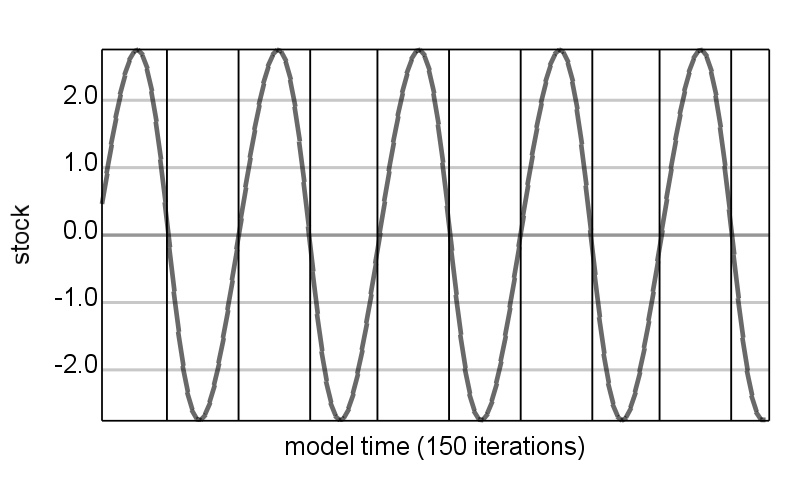
\includegraphics[width=0.9\textwidth]{ChapterConnectedModels/Figures/BT_modelday_3276_Transmission_singleFirm1_Wed-May-08-16_49_53-BST-2013__stock_vs_Time}}
\hspace{0.1}  
\subfloat[Good cost]{\label{fig:osc2}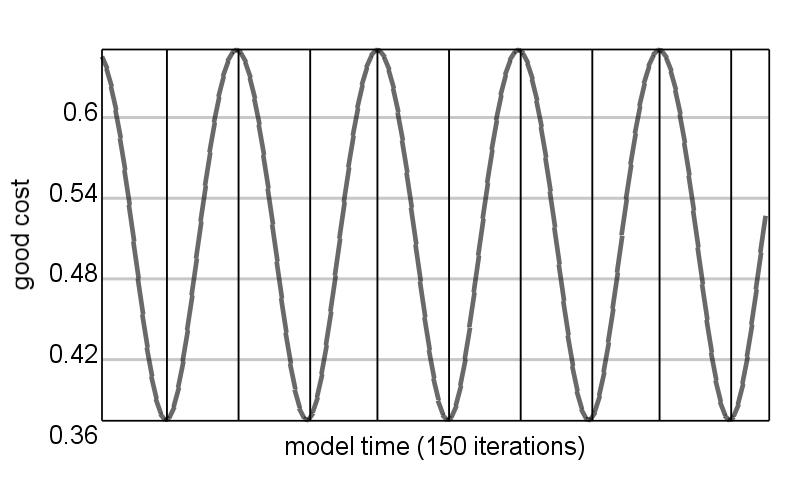
\includegraphics[width=0.9\textwidth]{ChapterConnectedModels/Figures/BU_modelday_3344_Transmission_singleFirm1_Wed-May-08-16_49_53-BST-2013__goodCost_vs_Time}}
\caption{Transmission belt model: a single Firm changing price to target zero stock. Vertical lines indicate where stock crosses the y axis. As stock hits zero, however, price is far from its equilibrium value and both stock and prices oscillate. \label{fig:TM1_oscillate}}%
\end{figure}

This is a version of a classic problem of harmonic oscillators that can be addressed by using damping (see e.g. \citealt{taylor_classical_2005} pp.172). The goal is not only to target zero stock, but to aim for both stock and price rates of change to be zero at the same point. The solution is relatively straightforward: target the first derivative of stock as well as raw stock levels. If price is made to aim for the point where both are zero simultaneously, equilibrium should be reached. In fact, adding a second derivative zero target can improve the targeting even further. 

Figure \ref{fig:TM1_damp} shows three model runs, this time using these extra first and second order targets. The `derivatives' are discrete differences in the model between timesteps. The first order derivative is the difference between stock at time $t-1$ and at $t$ and the second order is the difference between this first order result between timesteps. The target mechanism itself does not change: if $s + s' + s'' \neq 0$, price is changed in proportion to how far from zero it is, as described above: $\triangle p_g = (s + s' + s'') /x$ where $x$ controls the price change magnitude. If $s + s' + s'' > 0$, price is decreased and more stock sells. If $s + s' + s'' < 0$, price is increased and less is sold. 

Sub-figure \ref{fig:damp1} shows good cost for a single Firm / single Person run. Sub-figure \ref{fig:damp2} shows good cost for fifty Firms with fifty People, with initial good costs randomised between $0.1$ and $1.5$. Sub-figure \ref{fig:damp3} adds a distance cost to those hundred agents. It gives them random, static locations in $R^2$ so that People buy from Firms at a range of distances, with each position being unique. In the two runs without distance cost, the equilibrium price of $0.5$ is reached. It appears faster for sub-figure \ref{fig:damp2} (despite showing fewer iterations) because of the larger number of People: each time one of those People buys, it triggers a Firm's price response, so there are actually fifty such responses per Firm per timestep.

Figure \ref{fig:TM1_damp2} introduces an element of distance: agents' locations are randomised on an $R^2$ plane of one unit distance per side and goods are given a distance cost of $0.25$. The result illustrates a basic point about the transmission model: a stable equilibrium can be found with agents facing heterogenous costs from different spatial locations. The result is a spread of equilibrium good prices, as each Firm receives a different quantity of inputted time, and thus the equilibrium production level to maintain the zero stock target is different for each. Sub-figure \ref{fig:damp4} shows this result in more detail by correlating each Firm's good cost to the amount of time being contributed to it. This graph shows data from day $600$, which is the very right hand point of sub-figure \ref{fig:damp3}, at a point of stability. For a Firm with a production function exhibiting economies of scale, higher input levels increase per-unit output levels. In seeking to maintain a net-zero level of stock, lower prices are found to clear this higher-efficiency level of production - with the effect also of increasing Peoples' overall utility levels.

\begin{figure}[]
\centering
\subfloat[Good cost for One Firm, one Person buying]{\label{fig:damp1}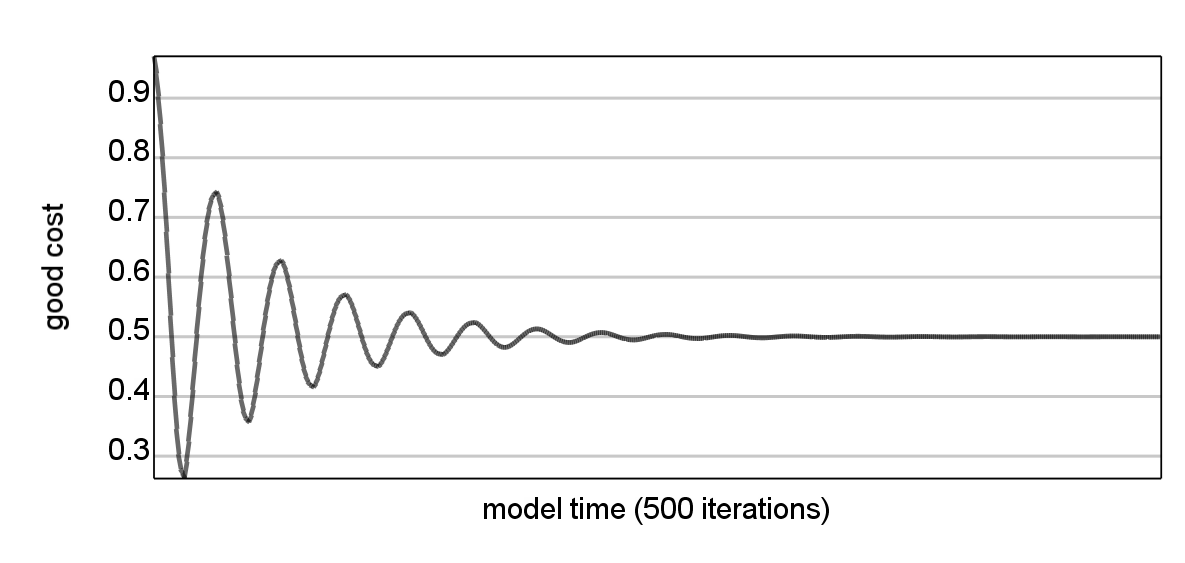
\includegraphics[width=0.9\textwidth]{ChapterConnectedModels/Figures/DG_modelday_941_Transmission_singleFirm1_Tue-May-14-09_37_25-BST-2013__goodCost_vs_Time}}
\hspace{0.1}
\subfloat[Good costs for fifty Firms, fifty People buying]{\label{fig:damp2}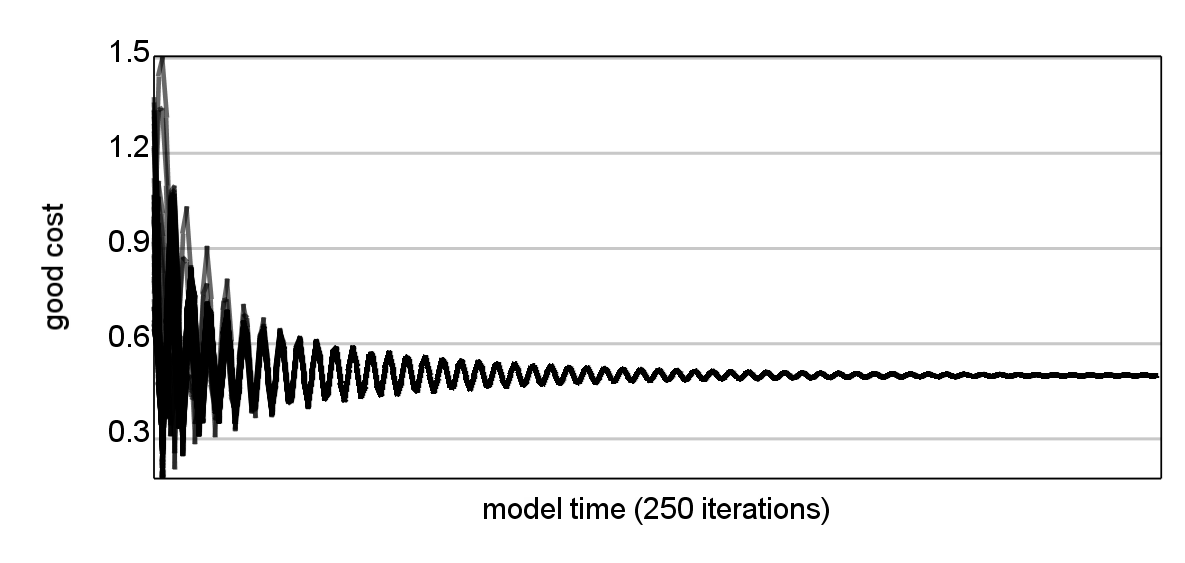
\includegraphics[width=0.9\textwidth]{ChapterConnectedModels/Figures/DH_modelday_533_Transmission_singleFirm1_Tue-May-14-09_39_47-BST-2013__goodCost_vs_Time}}
\caption{Transmission belt model: targeting the first and second derivative of stock as well as zero stock itself, `damping' the oscillations and achieving equilibrium. Example of single Firm and Person and Fifty Firms and People. \label{fig:TM1_damp}}%
\end{figure}

\begin{figure}[p]
\centering
\subfloat[Good costs for fifty Firms, fifty People buying, distance cost = $0.25$, random locations in an $R^2$ plane of 1 unit distance to a side. Showing damping of oscillations over model time.]{\label{fig:damp3}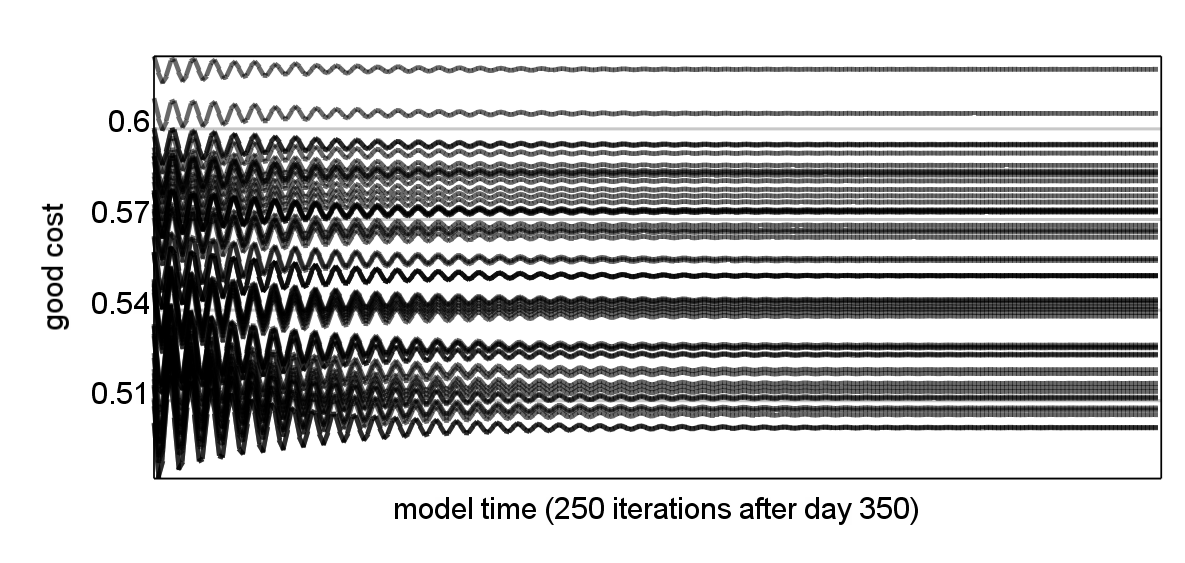
\includegraphics[width=0.9\textwidth]{ChapterConnectedModels/Figures/DI_modelday_516_Transmission_singleFirm1_Tue-May-14-10_11_39-BST-2013__goodCost_vs_Time}}
\hspace{0.1} 
\subfloat[From same model run, correlation of time contributed to each Firm versus their good cost at equilibrium, on day $600$ (very right of sub-figure \ref{fig:damp3}).]{\label{fig:damp4}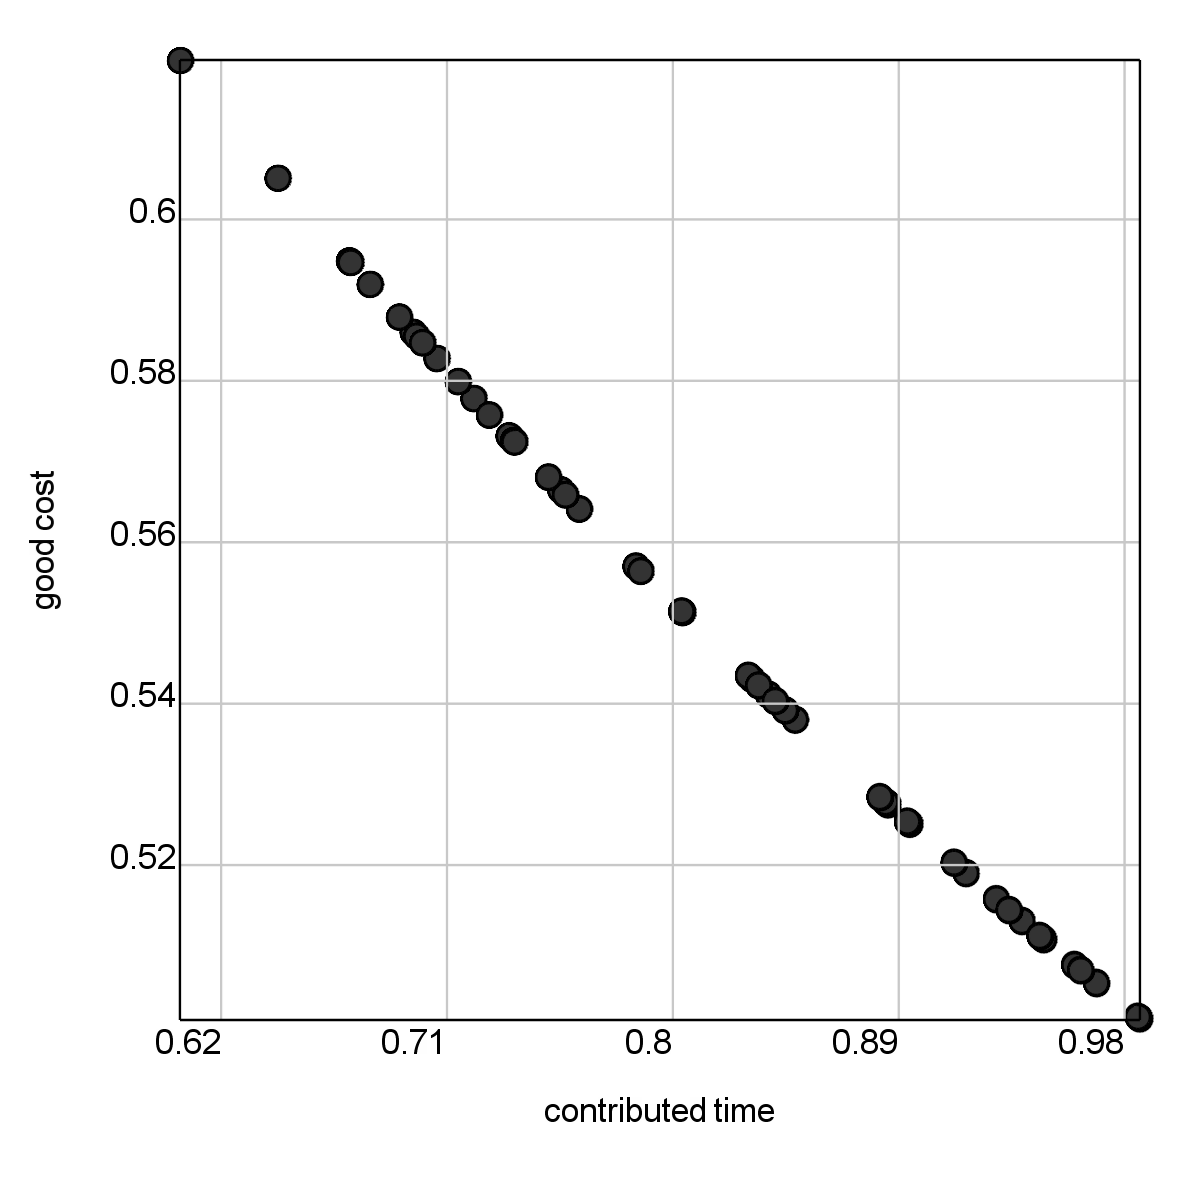
\includegraphics[width=0.9\textwidth]{ChapterConnectedModels/Figures/DN_modelday_943_Transmission_singleFirm1_Tue-May-14-11_44_10-BST-2013__currentContributedTime_vs_goodCost}}
\caption{Two graphs from the same transmission belt model run: fifty Firms, fifty People at random locations in $R^2$; distance cost = $0.25$. \label{fig:TM1_damp2}}%
\end{figure}

The classic equation for oscillation damping includes a term for angular frequency (ibid). Combined with a scaling parameter, in theory, the level of damping can be exactly targeted. The transmission model is `under-damped' - it oscillates before reaching equilibrium. Addressing this, however, would require detecting the angular frequency of those oscillations. While it is relatively straightforward to detect inflection points for many model runs, other runs produce complex interaction effects that make this detection process much more challenging. The solution used here is simply to manually set the scale of price reaction to stock changes for each model run using $x$, but it should be noted that this can impact on the exact point where Firms lose their grip on effective price-setting, as it determines the size of price swings - and consequently the scope for entering a positive feedback loop where stock targets are missed (see the next section).  

This example draws attention to another important feature of the transmission belt model. For model runs with a \textbf{single} Firm (and assuming space costs stay constant or at zero) production levels cannot change. People will always spend their entire budget on that one Firm. As this budget is also the total time available for production, this also does not change. With a single Firm, this means its production level is fixed: varying price only affects the amount of input that is bought. With more than one Firm, changing price \emph{can} effect production levels - but this is due to an externality. This externality also interacts with \gls{eos}, as the following section explains. 

\begin{figure}[]
\centering
\subfloat[Good cost, $20$ Firms]{\label{fig:tbmequil1}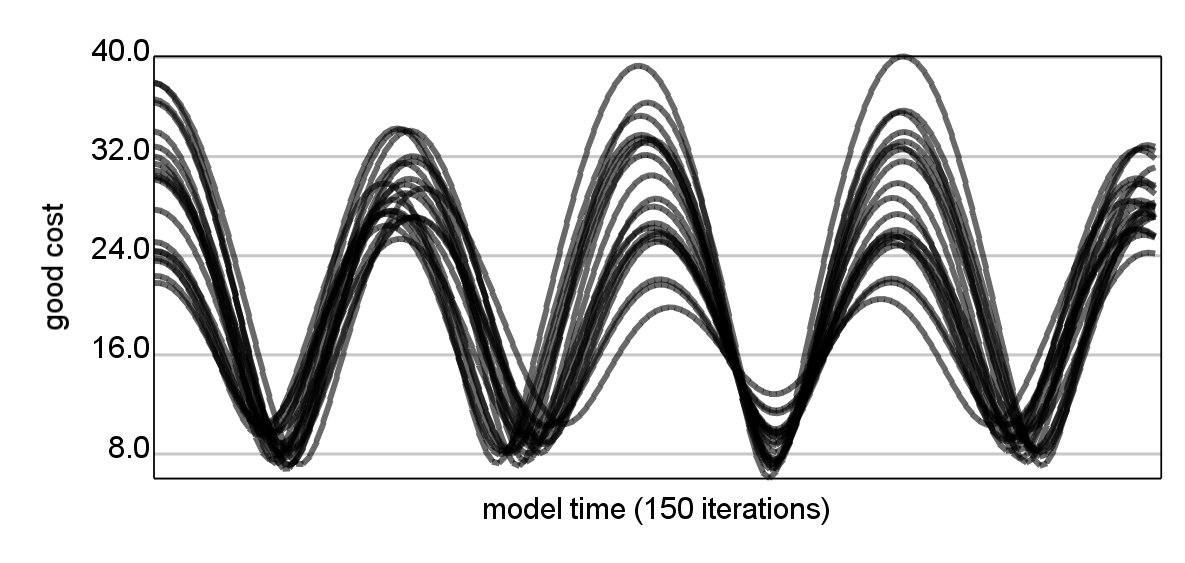
\includegraphics[width=0.9\textwidth]{ChapterConnectedModels/Figures/RV_modelday_279_EoS_LoV_noSpace_Fri-Jun-07-21_05_10-BST-2013__goodCost_vs_Time}}
\hspace{0.1}  
\subfloat[Utility, $100$ People]{\label{fig:tbmequil2}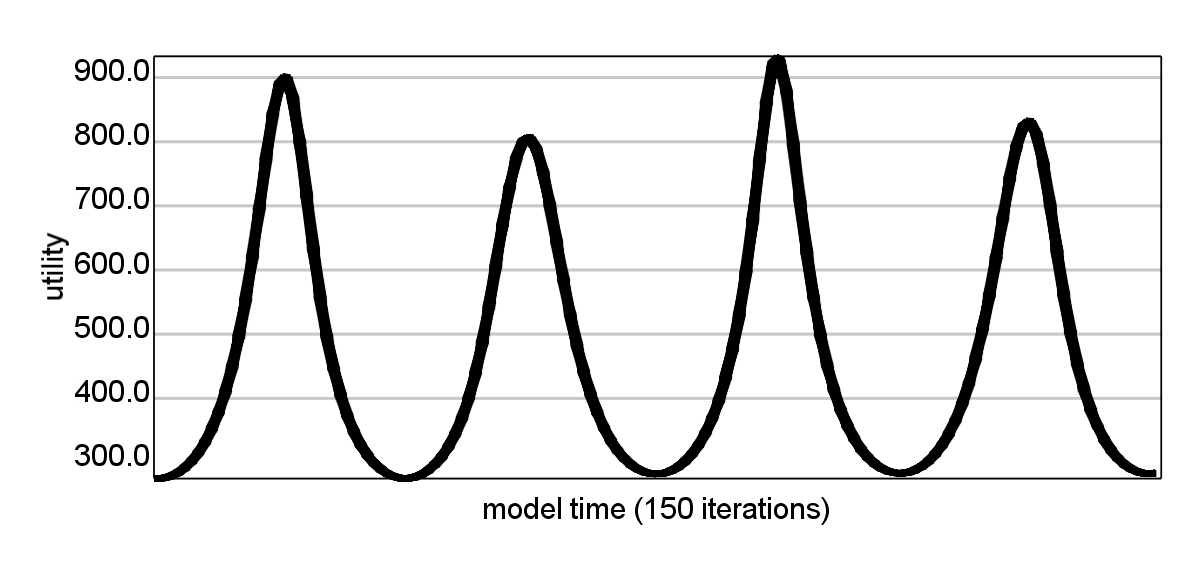
\includegraphics[width=0.9\textwidth]{ChapterConnectedModels/Figures/RW_modelday_359_EoS_LoV_noSpace_Fri-Jun-07-21_05_11-BST-2013__maxUtility_vs_Time}}
\caption{Transmission belt model, $20$ Firms, $100$ People, no distance costs. Firms are given randomised stock targeting magnitude response; result demonstrates People's utility equilibriates to a common value at each timestep, though it varies across model time. \label{fig:tbmequil}}%
\end{figure}

There is a final point that is useful to make while examining the basic stock-targeting mechanism: in the transmission belt model, People's utility equilibriates. In the presence of distance costs, if People are fixed at different locations relative to Firms (as they are for all presented models in this section) their utility is heterogenous simply because some agents can access goods more cheaply. All People's utility is umbilically linked; in a spaceless scenario where no intrinsic utility differences exist, this can clearly be seen, as People's utility remains identical. This is illustrated in figure \ref{fig:tbmequil}, which takes a $150$ timestep snapshot from the beginning of a model run with $20$ Firms and $100$ People. In order to contrast to People's utility, Firm's scaling parameter for the magnitude of their stock-targetting response to demand is randomised (sub-figure \ref{fig:tbmequil1}). The hundred People's utility levels are all shown in sub-figure \ref{fig:tbmequil2}: they are in lockstep, so appear as one line.

Utility does vary between timesteps - but People are following precisely the same path through time, having identical utilities at any one moment. While utility varies over model time, then, it stays in a dynamic equilibrium. Any possible improvement in utility is capitalised on by each Person at their point of decision, keeping the values umbically linked. Section \ref{sec:spacenwelfare} looks at People's utility in a spatial setting.

%This needs emphasising: good prices are \emph{not} set directly by Firms: they emerge through the price adjustment process of targeting a stock level. 
%That's completely wrong! What the hell am I talking about? Of course they set prices! They're just doing it based on granular feedback, and it looks like (well, is) a simple dynamic system, really. But it can still be framed as a `decision' just as much as other price decisions are. "Did my stock increase?" Etc.
\subsection{Markup and problems with competition \label{sec:markup}}

%So: that external effect point links to markup, I think? Hur. Well... the point being: this does support the Krugman point about prices being external in effect and its possible to see that directly. It just isn't possible to then get to any other of the core model mechanisms. I should write that up right now!
%This section also needs: basic impact of markup on prices and explanation of mechanism.
%As section \ref{sec:CMproduction} explained, in the \gls{coremodel} the mechanism for production equilibrium is variation in firm number. It is presumed (by setting profits to zero and deducing their number) that firms enter and exit the market depending on profit levels. 
In the \gls{coremodel}, a Firm's profit (or `markup') does not exist as a variable in the economy. It is part of the scaffold that drops away once the regional equations are reached. Its implied role is the signal to other firms about the level of demand: it is argued that, if profits are above or below zero, firms enter and exit the market until profits are driven back to zero again. A change in firm number is the \emph{only} way that production structure changes in the \gls{coremodel} and even then, the actual number plays no direct role in deducing welfare outcomes. 
%As always, Fujita \emph{et al.} are open about the oddness of these assumptions, noting as regards timings: ``we are assuming that the entry and exit of firms occurs very fast – so profits are always zero – but relocation of workers among sectors or locations occurs more slowly, with a dynamic we will model explicitly.'' (\citealt{fujita_spatial_2001} p.53)

This chapter does not examine Firm entry and exit: the number of Firms is set exogenously. It is potentially a fruitful avenue of investigation as it offers another way to examine changes in production structure. However, there are good reasons for leaving it out at this stage. Firstly, the models within this thesis have required agents to utilise only information they can collect from their environment. For a Firm to enter the market, having spied others making excess profits, it would need to be able to access that data directly. To know from a given price what profit another Firm is making requires also knowing their production output and markup. Starting to give agents this level of access to information takes the models into a different realm of knowledge and \gls{dmr}. It would not necessarily require a `master agent' watching global variables and adding or removing Firms appropriately; as section \ref{sec:coord_production} discussed, an evolutionary approach might add Firms randomly and allow them to attempt survival, while also allowing failed Firms (see section \ref{sec:markup}) to `die'. But the mechanics of entry and exit are complex, particularly for the transmission belt model where any change can cause perturbations large enough to knock other Firms over a `tipping point' (see below), causing runaway problems for the model dynamics. 

In the transmission belt model, Firms \emph{are} able to gain a profit - thus the first ingredient for an explicit Firm-level economic micromotive is present. But for this to provide Firms with complete economic motivation, they would need to be able to maximise that profit. In the \gls{coremodel}, profit maximisation involves simply finding the first order zero-point of a profit equation. In the transmission belt model, some explicit mechanism is required. This section explains how Firms in the transmission belt model can gain a markup and how that causes external effects. But it also outlines that, as the model stands, creating an effective competition mechanism is problematic.

The mechanism that a Firm can use for gaining markup is as follows. `Markup' is actually an amount of output they keep for themselves. A Firm sets a target amount of output they want to skim from each transaction and then uses price as a secondary targeting mechanism to reach it. This is a rather unique way to make a profit, so it bears re-stating: Firms' good price is \emph{dependent} on their markup target. The production target itself is set; the stock targeting mechanism attempts to achieve it, adjusting prices in the process. 

Achieving this is slightly awkward, as attaining a markup means that extra output must be produced \emph{constantly}. If a Firm simply aims for a higher stock target level and stops there, it is still net zero change over time. In order to get a markup, it needs stock to be increasing over time, and to take that increase for itself as profit. To do this, the Firm needs a markup level it aims for. This is then added to a moving markup target so that the Firm aims to skim a constant amount in a given time period. The stock target equation is altered to: $s + s' + s'' = mt$ where $mt$ is the moving markup target.
%\footnote{There are slight alterations to this in the code: it is easier to continue to target zero stock while shifting other values, but the principle remains the same.}. 
%Firms do not of setting prices directly. Instead, a
%Those are all potential directions for the model to take in future, but firm entry and exit does not form part of the thesis models.  Instead, the focus is on those areas of production structure the transmission model can naturally work with: the interaction of \gls{eos}, \gls{lov} and distance.
%It achieves a somewhat artificial outcome that is nevertheless useful for shedding light on the relationship between key production and consumption parameters.
%In the transmission belt model, Firms' 

Equilibrium good prices for Firms seeking markup are higher than the zero-stock clearing price. This higher price emerges as it targets the higher level of stock: it ends up charging extra and keeping a cut of the output. The external effect of this raised price is to drive demand to the second Firm. The way other Firms respond to this external effect depends on whether they have \gls{eos}. Without them, the extra demand they receive as input is linear with output change and the stock clearing price is the same. It is only in the presence of \gls{eos} that the external effect (beyond shifting demand) will be a change in stock-clearing price: it will become lower as a more-efficient production point is reached. 

Without economies of scale, any change in markup by one Firm will not change the absolute price of the other (dependent) Firm. It does change \emph{relative} prices as one Firm (the one making independent markup decisions) targetting higher markup leads to it finding a  higher equilibrium price - but it does not change the dependent Firm's price. When production scale is linear, demand does go up for their good but that is exactly matched by output level, so supply and demand for that Firm's good does not change.  Hence, the stock target remains the same and prices do not move. With \gls{eos}, however, changes in markup cause absolute price changes in both, as changes in demand cause both to shift up and down the \gls{eos} equation. This changes per-unit output, which changes the stock target level and then feeds through to equilibrium prices.

This is illustrated for a typical set-up in figure \ref{fig:TM1_markupEoS}. One Person buys from two Firms, with Markup for Firm 0 fixed at $0.1$. $\rho$ is fixed at $0.5$. The parameter controlling the scale of the curve in the \gls{eos} equation is swept from zero to one (shown on the x axis). The y axis shows the external effect that Firm 0's markup has on Firm 1's equilibrium price. For each value of the curve parameter, if there was no markup to consider, the equilibrium prices are straightforward: one Person buys 0.5 from each Firm. The values on the y axis show the difference between this `no markup' equilibrium price and the actual price the externally affected Firm equilibriates to, as they get more demand. Average price over the previous $500$ iterations are used, as the price fluctuates around its stable price daily due to the markup-seeking Firm constantly shifting its stock target. At zero, there is no curve: production scale is linear, so there is no change in the externally affected Firm's price. As \gls{eos} increases, this price gap becomes larger. (Note that $\rho$ is set at the level that keeps production from changing regime - see the next section for more on this.)
%A thought: the fact the EoS impacts on how markup works / where the boundary to working is. Actual EoS, that is, because of the external effect of price interaction.

\begin{figure}[]
\centering
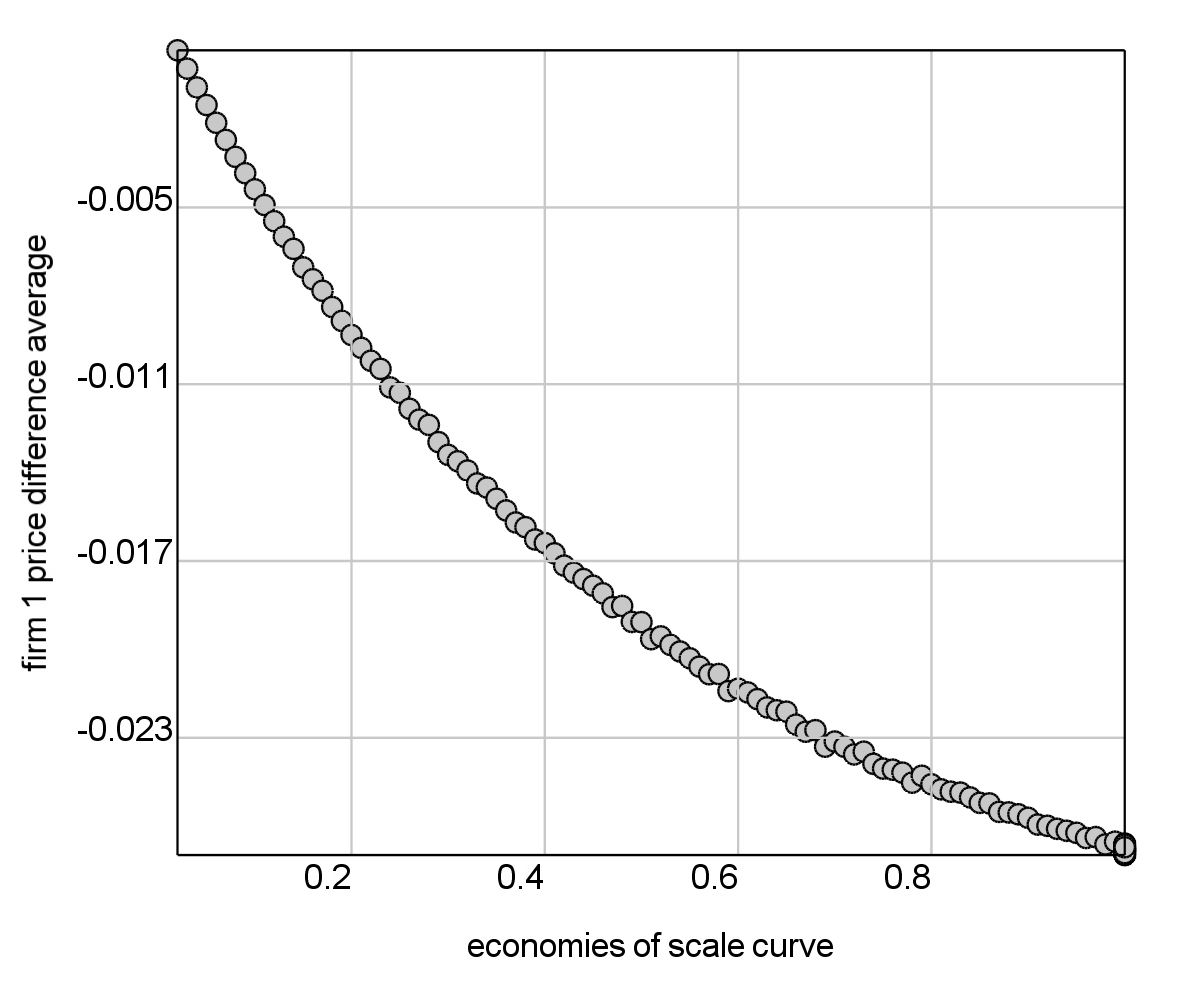
\includegraphics[width=0.8\textwidth]{ChapterConnectedModels/Figures/OV_modelday_112501_EoS_LoV_noSpace_Wed-Jun-05-18_03_48-BST-2013__EoS_Curve_vs_priceDiffFollow}}
\caption{Two Firm / one person transmission belt model. Firm 0 has a markup of $0.1$. $\rho = 0.5$. The x axis shows `economies of scale' curve swept from $0$ to $1$. The y axis shows, for the externally affected Firm, the difference between the normal equilibrium price (without markup) at that production scale and the price it finds. Average over previous $500$ iterations is used as the value fluctuates at short timescales. \label{fig:TM1_markupEoS}}%
\end{figure}

Figure \ref{fig:TM1_markupSweep} shows the effect of one Firm increasing its markup value (before hitting the `tipping point'; see below). It correlates the equilibrium prices of two Firms, with the \gls{eos} curve parameter fixed at $0.5$. Markup is swept between zero and $0.15$ for Firm 0. This shows up as a higher equilibrium price for its good as it aims for a higher stock target to keep a cut for itself. The external effect on the dependent Firm is shown on the y axis: its equilibrium price drops. It gets the demand driven away by Firm 0's higher price, which feeds into a more efficient production scale and thus a lower clearing price. In this case, the `raw' price is used, not an average over previous timesteps; this is to illustrate the volality of the price's oscillations, though the negative correlation is clear. 

These two figures, then, show that \gls{eos} and profit-seeking interact and cause effects external to Firms making decisions. This is a quite different dynamic to Firms entering and exiting a market, having seen the presence of profits. In the \gls{coremodel}, keeping the actual level of production itself static is an important simplification. Here, it is seen that in the presence of \gls{eos} one Firm changing its markup target pushes the two Firm's prices in opposite directions. The production structure of the whole economy is affected.

\begin{figure}[]
\centering
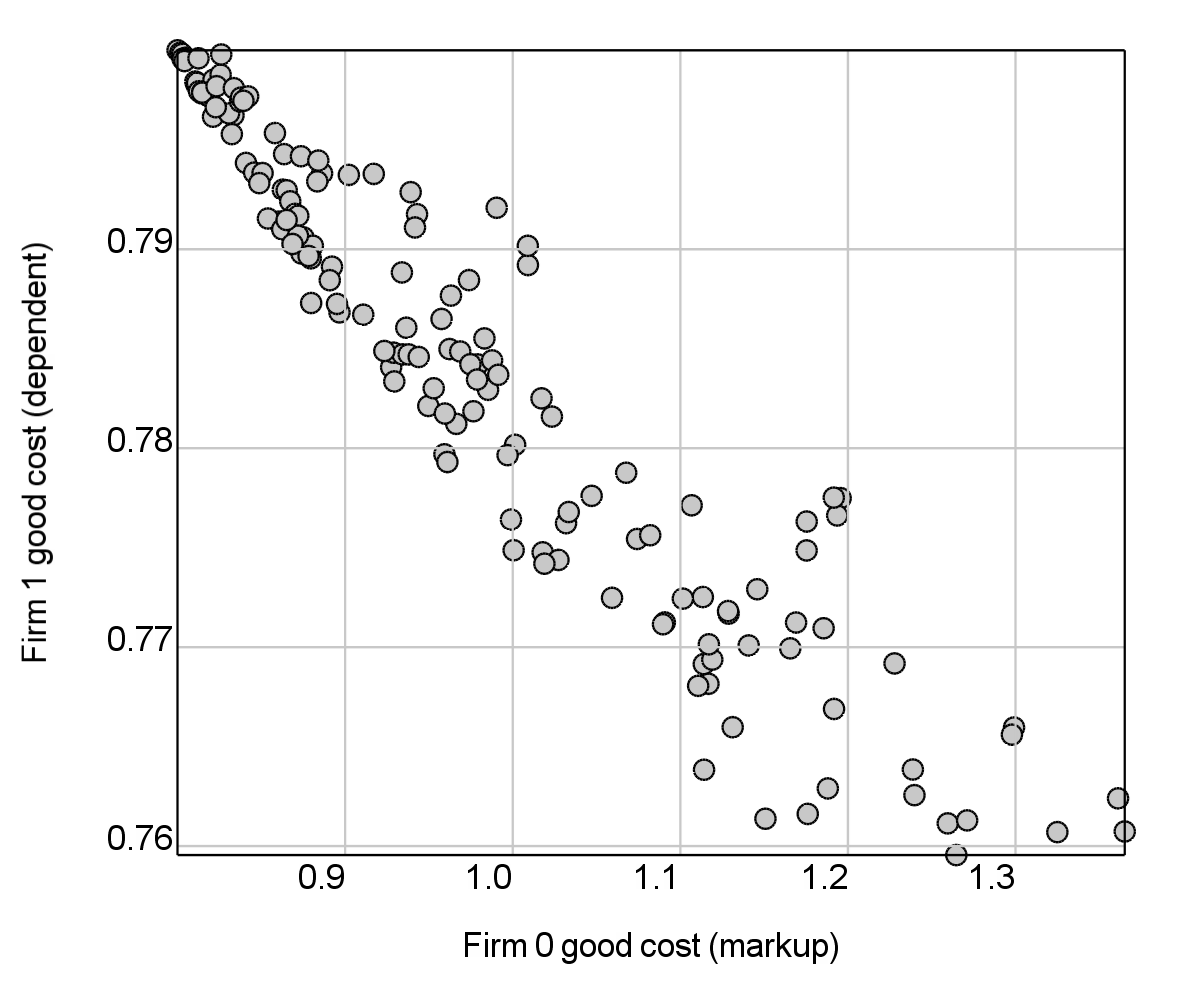
\includegraphics[width=0.8\textwidth]{ChapterConnectedModels/Figures/PV_modelday_153280_EoS_LoV_noSpace_Wed-Jun-05-19_00_02-BST-2013__goodCost_vs_goodCost}}
\caption{Two Firm / one person transmission belt model. Firm 0 varies markup between $0$ and $0.15$. $\rho = 0.5$, economies of scale curve $=0.5$. The Firm changing its markup (x axis) finds higher clearing prices, drives demand to Firm 1 (the dependent Firm), whose equilibrium price  drops. \label{fig:TM1_markupSweep}}%
\end{figure}

Firms can easily succeed in achieving a stable markup over time, then, for given markup target values. So there is a mechanism for achieving stable profits. But there are a number of problems with building on this foundation towards a fully competitive model. The first issue is \gls{dmr} related. In order to gain a profit, a firm needs to detect whether a change in markup target means `my action improved my profits' - but the transmission belt model is replete with conflicting signals. The model's oscillitory behaviour has been discussed; at present, angular frequency makes \gls{dmr} unmanageable. So this section concentrates on exploring the parameter space of price interaction through blind Firm behaviour - changing markup values directly and observing the effects both for the Firm changing its markup and the externalities on other agents.
%There is no logical barrier to Firms being able to `collude' to gain markup, but for \gls{dmr} reasons it is very difficult to make them able to seek even this level of profit-seeking. 

The second issue is a problem with Firms attempting to raise their markup: a `tipping point' exists that is disastrous for their stability and they are unable to pre-empt it. What causes the tipping point? One way into understanding the problem is to consider the role that \gls{lov} plays. Assume that $\rho = 1$ in a situation with two Firms, so both of their goods are completely substitutable. If their prices are equal, there is nothing to choose between them. However, if one Firm attempts to gain a markup, once their price is pushed up even marginally, demand for their good will drop to zero. 
%There are two ways of examining the problem.

So the ability of Firms to gain a markup is dependent on the value of $\rho$. In the model itself, as $\rho \rightarrow 1$, a Firm attempting markup reaches a price where it can no longer approach its stock target. This gap between their stock target and what they are able to achieve in production produces a constant pressure to change their price in order to try to get back to the target. The inability to move towards it only reinforces its price changes, and it enters a positive feedback loop: further price increases lock in its unaffordability and drive production to the other Firm. Figure \ref{fig:TM1_markupTippingPoint} makes clear an important feature of this tipping point: it correlates to $\rho$. Why is this? $\rho$ controls elasticity of substitution, thus the effect of any change on price. For higher values of $\rho$, as goods become more substitutable, People are less reliant on \gls{lov}: a change in price becomes a stronger signal for the other Firm. In this model run, $\rho$ is swept from $0.1 < \rho < 1$. One of two Firms slowly increases the markup it aims for (this markup is shown on the x-axis). At a certain price, it reaches the tipping point. Each increment of $\rho$ is triggered when this happens: the model is reset and run again, and one Firm again attempts to incrementally seek profit. (Two People are used in this run to indicate the basic dynamic functions the same as for one.)
%One of the two Firms (Firm zero) slowly increases its markup until it hits a `tipping point' where it can no longer effectively target a stock level and its price enters a positive feedback loop. This is taken by the model as the signal to parameter-sweep $\rho$:  it resets the Firms and runs again, for values of $0.1 < \rho < 1$. The stable markup value achieved before the feedback starts is graphed against $\rho$.

\begin{figure}[]
\centering
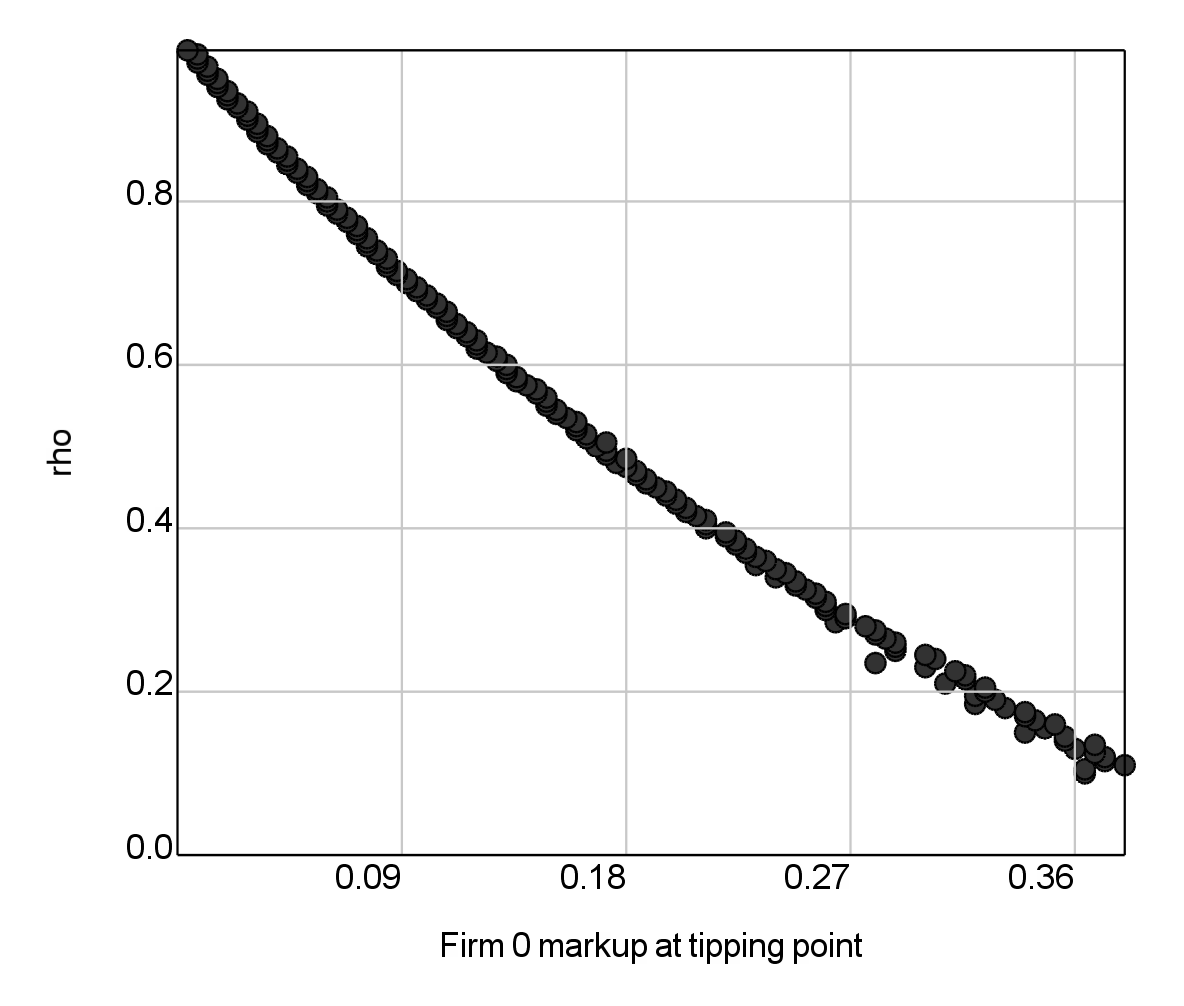
\includegraphics[width=0.8\textwidth]{ChapterConnectedModels/Figures/CS_modelday_1479445_Transmission_singleFirm1_Fri-May-10-16_05_52-BST-2013__markUp_vs_rho_NO_EOS}}
\caption{Two Firm / two person transmission belt model. The graph shows Firm zero's markup target correlated to $\rho$ , with datapoints taken when the Firm hits a `tipping point'; there are no economies of scale. \label{fig:TM1_markupTippingPoint}}%
\end{figure}

There appears to be a more fundamental reason why any competitive outcome, in the current model set-up, is not possible. All Firms are incentivised to seek a stable markup but, while the external effect of one doing so is to move demand to others, that demand has no impact on other Firms' profits: each Firm has its own stock target and moves prices to meet it. So, each Firm must separately attempt to raise its markup target if it wants a profit. The dynamic created is a ratchet effect: each individual Firm is able to take extra slices of production for themselves, right up to the point where People are no longer able to afford to buy the remaining output that Firms do not keep as profit - at which point, there is no incentive to work and the system collapses. Note again that People have no exogenous options for spending their time and thus no effective sanction that could produce competitive behaviour in Firms. Even if goods' cost is exhorbitant, they will pay it, as no other options are available to their utility functions and a sliver of utility is better than none. 

To summarise: there are only two possible outcomes for Firms attempting to seek profit, as the model is currently structured. If Firms collude, or succeed in following a collusion-like pattern through independent actions (implicit collusion), they can squeeze profit out of People right up to the point where People can no longer afford to buy anything at all. Or, if one or more Firms attempts to get markup, this is sustainable up to a point, but then tips over into a positive feedback loop between the external effect of lowered prices for others and the profit-seeking Firm's inability to use price to target their new stock level due to having lost too much demand. Missing their target causes them to continually increase their price, permanently compounding their error. 

As the transmission belt model stands then, there is no stable competitive outcome that can emerge through Firm interaction alone that allows for Firms seeking profit. Firms' price signals \emph{can} be used for targeting stock level and can function as an effective distributed mechanism for finding equilibria across all agents. 

%\begin{figure}[p]
%\centering
%\subfloat[Firm zero seeks markup at varying values of $\rho$; no economies of scale]{\label{fig:markUp}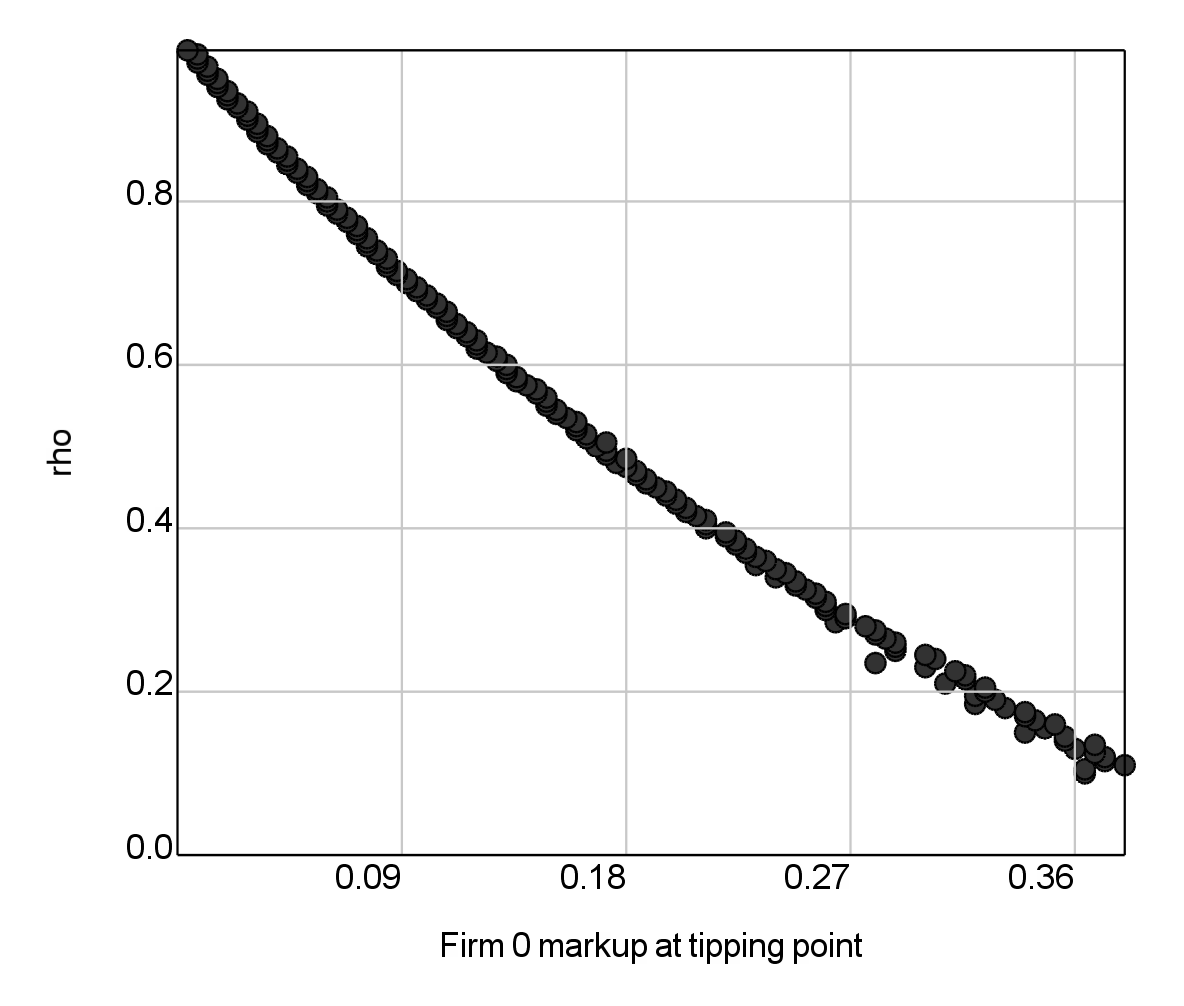
\includegraphics[width=0.8\textwidth]{ChapterConnectedModels/Figures/CS_modelday_1479445_Transmission_singleFirm1_Fri-May-10-16_05_52-BST-2013__markUp_vs_rho_NO_EOS}}
%\hspace{0.1}
%\subfloat[Firm zero seeks markup; economies of scale cause external price effect. Two firms' prices correlated.]{\label{fig:markUp}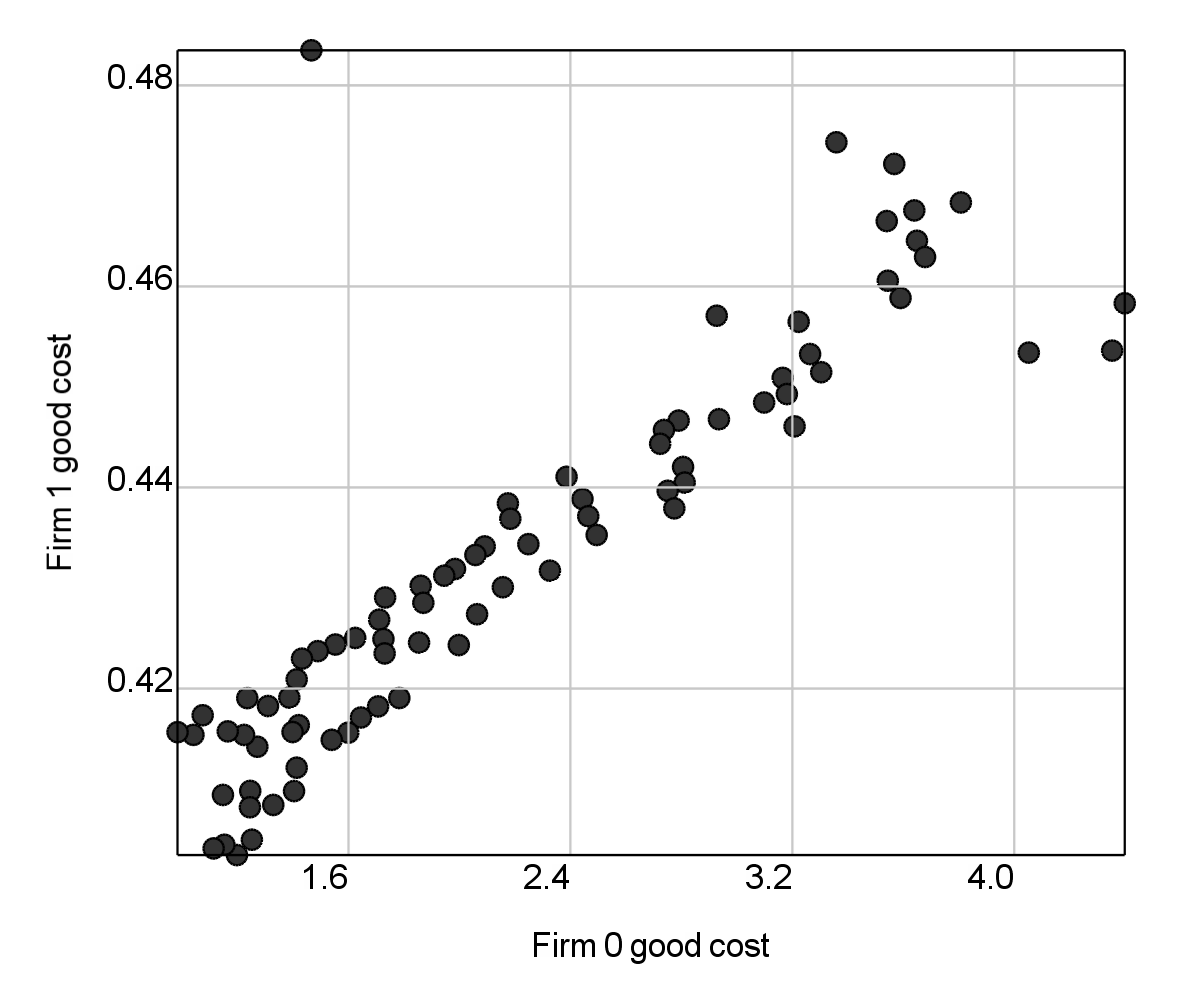
\includegraphics[width=0.8\textwidth]{ChapterConnectedModels/Figures/EC_modelday_1703184_Transmission_singleFirm1_Tue-May-14-14_26_13-BST-2013__goodCost_vs_goodCost}}
%\caption{Two Firm / two person transmission belt model. The first figure correlates Firm zero's price as it raises its markup target. Data is shown at the tipping points, correlated to $\rho$; there are no economies of scale. The second includes economies of scale and shows the external effect of Firm zero's price changes on Firm one's price, driving it down. \label{fig:TM1_markupTippingPoint}}%
%\end{figure}
%\cmt{This figure doesn't quite fit! Move things, reduce the caption.}
%\cmt{Be sure to clarify what the markup value on the graph is: aiming for a marked up STOCK level.}
\subsection{Interaction between economies of scale and love of variety \label{sec:lov_vs_eos}}

\begin{figure}[p]
\centering
\subfloat[Two Firms: output per unit of input time]{\label{fig:eoslov1}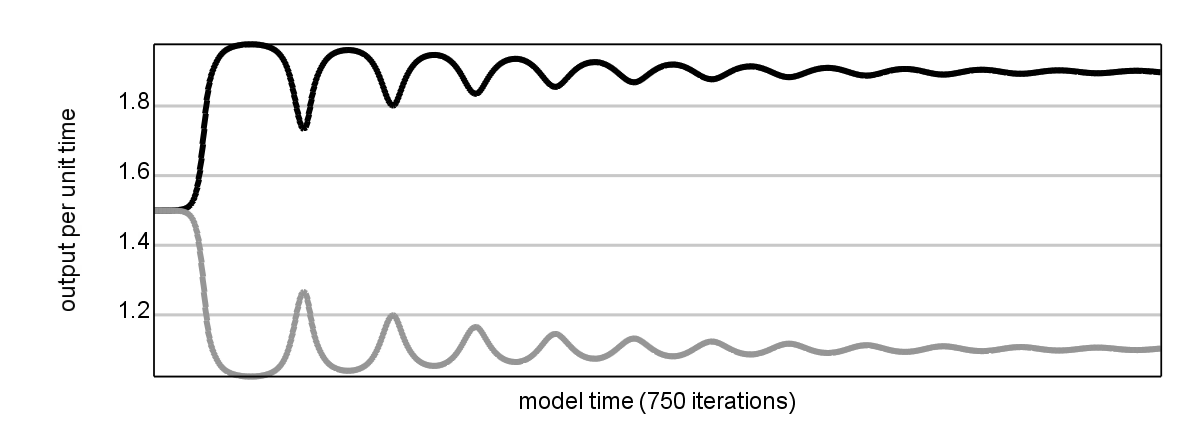
\includegraphics[width=0.85\textwidth]{ChapterConnectedModels/Figures/FX_modelday_3375_EoS_LoV_noSpace_Fri-May-17-11_09_25-BST-2013__Output_per_unitTime_vs_Time}}
\hspace{0.1}
\subfloat[Two Firms: stock levels]{\label{fig:eoslov2}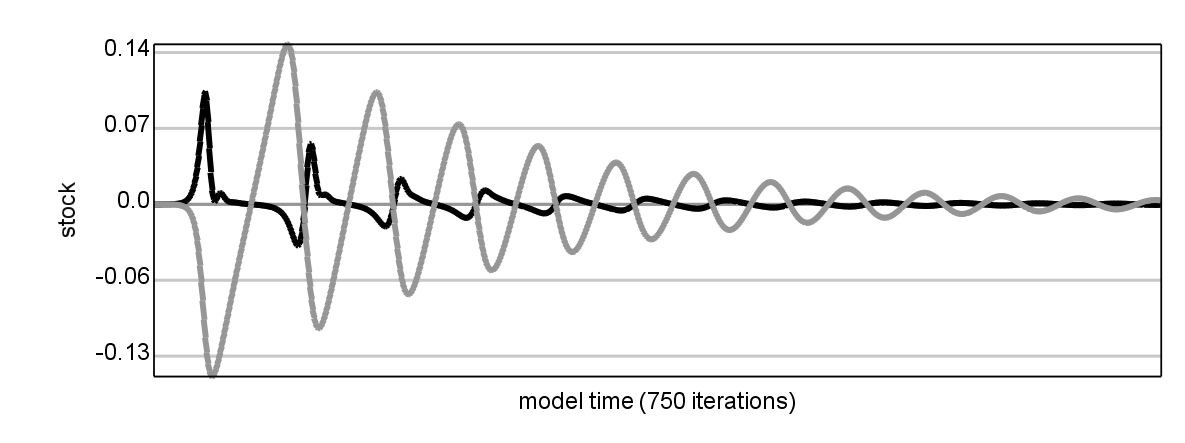
\includegraphics[width=0.85\textwidth]{ChapterConnectedModels/Figures/FY_modelday_3493_EoS_LoV_noSpace_Fri-May-17-11_09_27-BST-2013__stock_vs_Time}}
\hspace{0.1}
\subfloat[Two Firms: good cost]{\label{fig:eoslov3}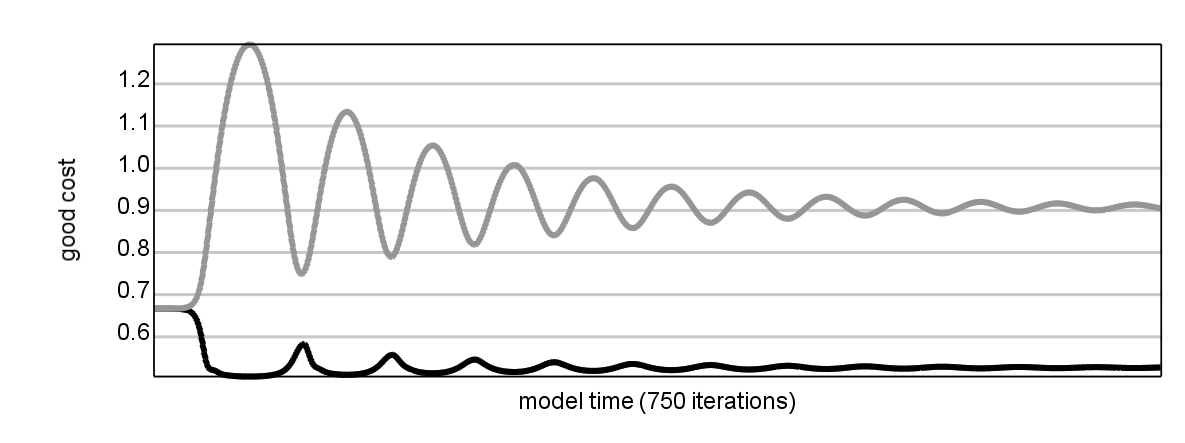
\includegraphics[width=0.85\textwidth]{ChapterConnectedModels/Figures/FZ_modelday_3566_EoS_LoV_noSpace_Fri-May-17-11_09_29-BST-2013__goodCost_vs_Time}}
\hspace{0.1}
\subfloat[Person's utility]{\label{fig:eoslov4}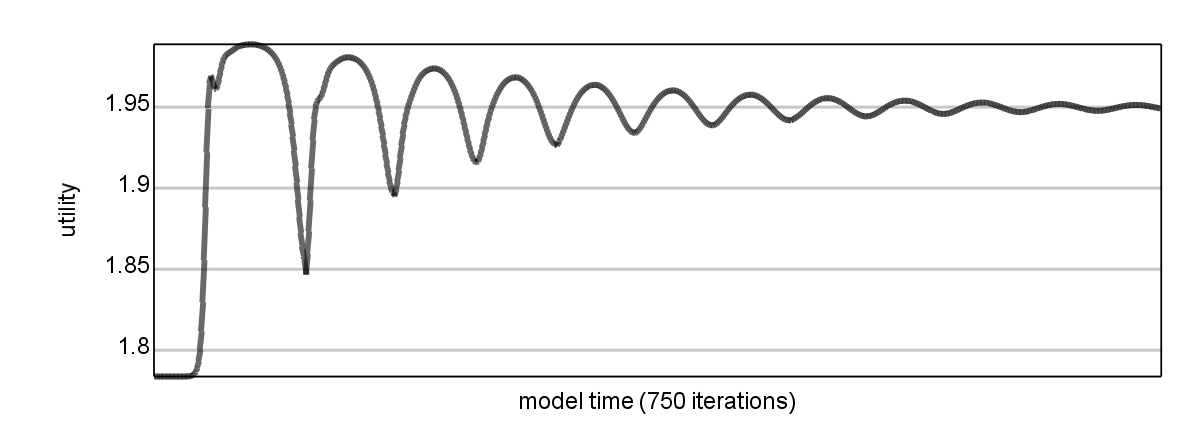
\includegraphics[width=0.85\textwidth]{ChapterConnectedModels/Figures/GA_modelday_3655_EoS_LoV_noSpace_Fri-May-17-11_09_30-BST-2013__maxUtility_vs_Time}}
\caption{Two Firm / one Person transmission belt model moves between production regimes as $\rho$ crosses substitutability threshold. Black and grey identify the two Firms in the first three graphs. $750$ Model `days' shown after transition from $\rho=0.73$ to $\rho=0.8$. \label{fig:TM_eoslov_tippingPoint1}}%
\end{figure}

%\cmt{``Krugman’s trade theory showed how trade patterns seen in the real world can come about with no fundamental initial differences''. Also no fundamental differences in mine: connect that to the basic LoV/EoS thingyo.}


%If you have actual EoS, there is a trade-off between scale of production and LoV that might mean one or more efficient producers can get lock-in. That's probably the most important thing to say. I haven't yet shown that can block the entry of new Firms but it's bound to have an effect. I think I did show 1 more firm entering did knock it out of EoS, but gonna have to leave open for now.

Continuing with a model with no distance costs, this section outlines how \gls{eos} and \gls{lov} interact in the transmission belt model. The model uses explicit \gls{eos}: Firms have a production function where output per unit input increases with input. Consumers have an entirely separate \gls{lov} utility function. This allows interaction between them to be investigated. This section demonstrates that, in the transmission model, the interaction of \gls{eos} and \gls{lov} can determine the whole model's production structure. In contrast to the \gls{coremodel}, distance is not required for a shift between model regimes to occur. Within the parameter space defined by \gls{eos} and \gls{lov}, agents can find two distinct production regimes. In one, \gls{lov} dominates and production is spread out among all  producers symmetrically. In the other, the \gls{eos} effect dominates, and that symmetry is broken. While the transition is `catastrophic', changes to relative production scale exist beyond that point, determined by \gls{lov}: the state of the model is not simply binary. If the smooth \gls{eos} function has zero curve and production is linear, any change in $\rho$ has no effect on price, for the reason mentioned in the previous section. 

This model example reduces complexity even further by only using one Person buying from two Firms. This makes it possible to compare to a very simple deductive version with the same output values and results, enabling a clear view of how the transmission belt model's agents move between production regimes. 

Section \ref{sec:CMproduction} explained that, in the \gls{dxs}, economies of scale at production level are subsumed into two things: the \gls{lov} parameter (or its mirror, the elasticity of substitution parameter $\epsilon$) and a market structure argument that reduces economies of scale to the entry and exit of firms. It is a very powerful set of deductions that allow everything else that follows a solid mathematical foundation. As Brakman \emph{et al.} (\citeyear{brakman_new_2009} p.106) note, ``internal economies of scale are not absent... but show up in only in a rather special way.'' The \gls{coremodel} does contain parameters for production level \gls{eos} in its `scaffold', but the final model is not sensitive to their value in any way. Indeed, with the normalisations mentioned in section \ref{cm_normalisations}, they are analysed away. 
%So this masks the fact that they can interact. Which is almost poetry, really.
%The emergence of one efficient producer can be enough to knock the other over the tipping point, if their attempt to correct their price is too severe. This locks the efficient producer in completely. At certain values, however, the less efficient producer can keep a toe-hold in the economy. 
%Note: it requires a slight initial difference, as the CM would if it worked that way! Setting prices the same to start with locks the model in, it can't change. Starting from random prices, allowing equilibrium to emerge allows a slight enough decimal point difference between prices (how much?) that the model can move between equilibria.

To begin with the model output itself, using all the features described in the sections above, figure \ref{fig:TM_eoslov_tippingPoint1} shows what happens for the two Firms and one Person at the point where \gls{lov} drops low enough to tip the model over into one efficient producer. The change in value of $\rho$ that causes this (from $0.73$ to $0.8$) is not visible - see below for more on this - but rather, the story of what happens is shown through the four sub-figures. The first (\ref{fig:eoslov1}) shows each Firm's output per unit of input time. As more time feeds into one of the two Firms (identified by the black line), it produces at a more efficient scale: output per unit input grows. 

Underpinning this is People's demand separating out from a symmetric split between the two and entering a feedback between price and efficiency (this is the essential part of the model and is explained in more detail below). As a consequence (\ref{fig:eoslov2}), this Firm sees its stock level increase initially, while the second firm loses stock as it is now producing at a less efficient scale. It takes some time for both Firms' price reaction to take effect (\ref{fig:eoslov3}): the end result is a more efficient producer able to charge a much lower price to maintain net-zero stock, effectively locking it in as the favoured site of production. The final sub-figure (\ref{fig:eoslov4}) shows the driver for this change: the Person finding that shifting their demand to the higher-efficiency producer increases their utility. 

\subsection{Tracking down the `transmission belt' \label{sec:transmissionbelttrackinz}}

What is causing the shift between these two stable states? The problem can be boiled down into its component mathematical parts, allowing an examination of the `transmission belt' between production and utility in its simplest form. There are four pairs of variables to consider (with one set each for the two Firms): 

\begin{itemize}
	\item The price each Firm is charging for a unit of output ($p_0$ and $p_1$).
	\item The optimal amount of each good demanded by the Person ($c_0$ and $c_1$) based on those prices being input into their \gls{ces} function.
	\item The quantity of stock produced by the Firms ($f_0$ and $f_1$) based on how much time the Person exchanged for their optimal amount. Their time input is just their optimal amount multiplied by the price they paid for it. (The `price' is the amount of time they must pay for that optimal amount.)
	\item The difference between the demanded stock ($c$) and produced stock ($f$), $c_0 - f_0$ and $c_1 - f_1$. 
\end{itemize}

To understand how the dynamic works, a useful question to ask is: what makes the model move away from its symmetric equilibrium? Equally, what can hold it there if the variables are perturbed away from symmetry? The coded model suggests that, for values of $\rho$ below $0.75$, demand remains symmetric across the two Firms, whereas if $\rho > 0.75$ (and if there is a slight perturbation in initial values) one more-efficient producer emerges. 

The model's values can be deduced around this transition point. When production is symmetric, time is split evenly between the two Firms: $0.5$ for each. So stock output using the smooth \gls{eos} function is $f = t^2 + t = 0.75$.  For a production equilibrium, that $0.75$ needs to be `cleared': the stock must remain at net zero, so two lots of $0.75$ must be sold. If a Person is paying $0.5$, it has to cost $p =0.66'$. (If it costs $0.66'$ for a unit of good, paying $0.5$ gives the person $0.5/0.66' = 0.75$.) 

So $p=0.66$ is the equilibrium price at symmetric equilibrium. The goal is to discover what happens when prices are perturbed by a tiny amount from that equilibrium: do they return back or do they move towards another stable equilibrium? This is where the last pair of variables come in: the difference between the optimal demanded amount and the output produced. With slight differences from symmetric equilibrium prices, these two values do not quite match - thus the market is now out of equilibrium as it cannot completely clear at those prices. 

This mismatch is a logical outcome of the smooth \gls{eos} function and the clearing price. If price is slightly lower than the stock clearing amount for a Firm, demand will be higher - and because \gls{eos} can be gained smoothly, any tiny amount of difference in input leads to a larger input/output ratio, however marginal. Due to this mismatch, Firms must find a new clearing price. Section \ref{sec:stocktarget} has already explained how this is accomplished in the transmission belt model, in a situation where demand may be coming from many different People and places. In this one-Person case, the job is more transparent: there is a simple difference between the single Person's demand and the amount produced and this allows the two Firms to make a price adjustment to seek a stock-clearing value. 

This example can be input into a spreadsheet to demonstrate what role \gls{lov} plays. This removes all coordination and agent timing concerns to show the underlying dynamic as clearly as possible. The slight difference between $c$ and $f$ produced when prices move a little from the symmetric equilibrium implies a price change polarity for Firms to use. This can be described as a simple differential equation: $p_n' = f_n - c_n$. As explained in section \ref{sec:ace}, this is a Leijonhufvud-like `law of motion': if demanded stock is more than produced stock, price is going up to reduce demand; if demanded stock is less than produced stock, price is going down to reduce demand. In the spreadsheet, this change is just a very small constant at each step. 

The result is to show whether or not the Firms' price adjustments converge back to symmetry or diverge to a new equilibrium, testing whether the symmetric equilibrium is stable at given values of $\rho$. Figure \ref{fig:spreadsheetOutput} shows the output from the spreadsheet for two different values of $\rho$ on either side of the symmetric/divergence point\footnote{This spreadsheet is included in the downloadable model `zip' file via the link provided in the code appendix (\ref{apx:modelcodeoverview}).}. Where $\rho < 0.75$ in sub-figure \ref{fig:spreadsheet1}, the fixed price adjustment quickly converges back to stable symmetric prices, oscillating around that point due to the fixed adjustment constant used in the spreadsheet. Sub-figure \ref{fig:spreadsheet2} shows one producer emerging as the more-efficient, stabilising at a new pair of equilibrium prices.

%contains constrained optima, (twice if one counts it being used to calculate the time the Person contributes)
Looking at only one Person and two Firms in this simple example helps make clear exactly where the `externality' is doing its work: through the constrained \gls{ces} utility function. The differential equation describing Firms' price changing behaviour, $p_n' = f_n - c_n$, contains the constrained optimum good amount in $c_n$. The \gls{ces} function contains the price of the good being bought \emph{and} the price of all others - just a single other good, in this case, but it still means changes in the price of one always impact demand for the other, as there is a finite pot of demand. The scale of the elasticity is controlled by $\rho$. In the spreadsheet example, the `external' effect is not a matter of timing or interaction between Firms, as both Firms make their price decisions simultaneously. It is the impact those price decisions have within the Person's \gls{ces} function on the next step that encapsulate the externality. If one Firm changes its price unilaterally, this will still impact on demand for the other Firm's good - but via the action of the Person's utility function.
%For an arbitrarily small initial difference, $\rho$ determines at what point adjustments to price succeed in bringing demanded stock back into line with the amount produced through the smooth \gls{eos} function. In the spreadsheet example, the two Firms make a simple binary choice: if $f1 - c1 < 0$ then demand was too high and price is reduced by a set amount; if $f1 - c1 > 0$ the reverse action is taken. The size of the adjustments is unimportant: it is the magnitude of the difference between demand and production at each price that determines the path to equilibrium.

\begin{figure}[]
\centering
\subfloat[$\rho = 0.73$]{\label{fig:spreadsheet1}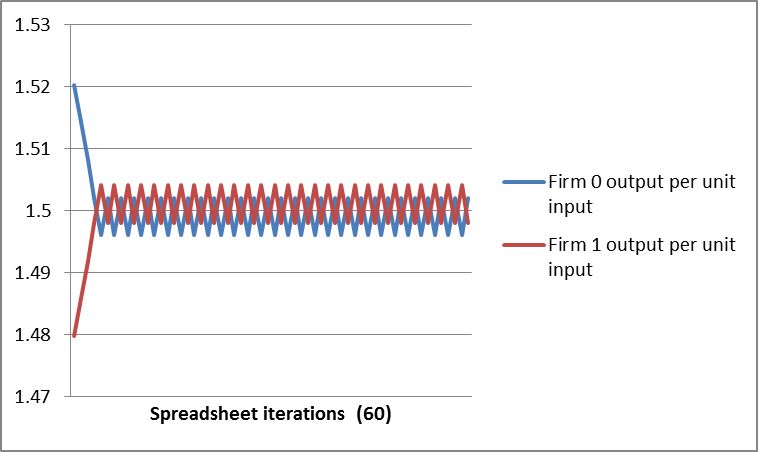
\includegraphics[width=0.85\textwidth]{ChapterConnectedModels/Figures/TBM_convergingSpreadsheet}}
\hspace{0.1}
\subfloat[$\rho = 0.8$]{\label{fig:spreadsheet2}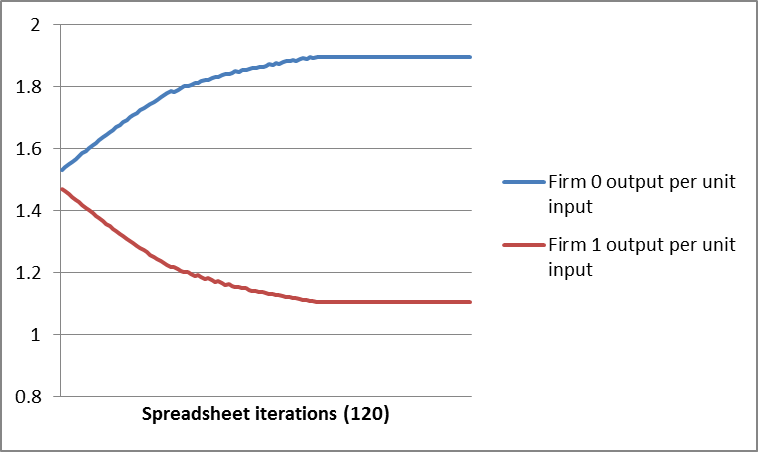
\includegraphics[width=0.85\textwidth]{ChapterConnectedModels/Figures/TBM_spreadSheetSpreading}}
\caption{Spreadsheet output of Two Firm / One Person example. If $\rho > 0.75$ the symmetric equilibrium is not stable: a slight difference in price leads to feedback to one, higher efficiency Firm and one lower. Note: $60$ iterations are shown in (a) as convergence happens quickly. \label{fig:spreadsheetOutput}}%
\end{figure}
%\cmt{Spreadsheet graphs in connectedmodels folder; EoSvsLoVExcelModelDanOlner2013.xlsx. Leaving for now until I've nailed what I'm doing with *all* excel graphs (style, colour etc) to avoid extra work. These two are placeholders.}

Though the transmission model is designed to handle complex spatial demand situations, this simple example illustrates how the outcomes are driven by the underlying economic behaviour and the interaction between Firms' production functions and an `externality' coming from elasticity of substitution between Peoples' good demand as $\rho$ changes. The tiny price difference required in this non-spatial version is, at root, also responsible for outcomes in the spatial examples used in the following sections. 
%\cmt{I should show: in equilibrium, difference all values of rho makes. To show it isn't just binary, there are price differences on both sides. So e.g. inputting range of rho values into the spreadsheet, pulling values out, or coding a simple version to do that.}
%And have I also really explained how come when rho is moving towards higher substitutability it happens to find its way to the more beneficial production arrangement? That's still something of a small miracle. I don't think there is, perhaps, any deeper explanation except the difference between demand and production level is led by this difference in rho, producing a feedback that pushes the model towards the more efficient producer.
%But of course that needs tempering: in a situation that had Firms with functioning micromotives, would that outcome still hold? I'm going to have to leave that as an open research question. But it's a tantalising finding nonetheless, and one that the ABM can do and other approaches cannot.
%Oh: a very obvious point that needs making. DXS can't do that. It assumes a symmetric outcome. The transmission model suggests the possibility of catastrophic shifts of production (while still maintaining other producers) even in a single region. Which is to say you don’t actually need space for increasing returns to lead to catastrophic outcomes.
%and a second where, through price signals from producers, agents discover a route to higher utility through increasing input into a small subset of producers, taking advantage of \gls{eos}. 
%Which is important given that DSX/CM subsume all that and EoS becomes hidden.
%Before introducing space...
%Ach, I had another important thought about that. Which was...? It was something to do with the fact that the model can find different production regimes even in a spaceless model.

\section{Introducing space into the transmission model \label{sec:TM_space}}
%May also require some "static" demand a la agriculture sector - though may not. Depends if Firms can move. They can't - they have no separate economic motivation to do so. Their stock target can't help them. I can lump them together (a Firm follows a Person)... which we could show can lead to the core-periphery dynamic with just EoS.
%That's an important point about market structure there: the same micromotive should drive price setting as well as location setting. Without it, the model is incomplete. I'm down with saying that. 
%I also want to say: I don't want to minimise the market structure argument made for the core model firms. It may be implicit but it is "real" all the same, cf. Fowler.
%Given all that, what do I gain from making a two-region version that includes Person movement? If manufacturing cannot agglomerate, what are we looking at, even? Well: if we leave manufacturing evenly split, agglomeration can still occur through EoS alone. Again, there's that caveat: what would the market structure implications be? One might speculate that if a Firm has lock-in, no market entry is possible. 

Section \ref{sec:stocktarget} used an example involving random spatial locations. It showed that, if agents have heterogenous location (and thus each Person faces a different set of good prices and each Firm a different quantity of demand) the transmission model is able to find a set of stable equilibrium prices for all Firms. But what role does distance play in the interaction of model variables and the transition between production equilibria? This section examines this question by following the example of the \gls{coremodel}, using the simplest possible representation of distance between two discrete regions. There are three model examples in this section illustrating essential points about the effect of distance in the transmission belt model:

\begin{enumerate}
	\item Keeping People's location static, with one Person in each of the two regions, two production regimes are determined by \gls{lov}, as in section \ref{sec:lov_vs_eos}, but distance cost can also determine the transition between regimes.
	\item Allowing People to move, the interaction with \gls{eos} locks the resulting emergent region with no way back: a `black hole' outcome.
	\item Two Firms per region, with two People static again, one per region. Four different kinds of production regime are possible by varying $\rho$ and distance cost, demonstrating heterogeneity within regions as well as between them.
\end{enumerate}
%One region can emerge as the chosen site of efficient production, but with symmetric production for the two Firms in that region. At lower \gls{lov}, a single efficient Firm within that region can emerge, breaking the symmetry


Varying rho alone in the presence of distance costs has a direct effect on outcomes (where in the spaceless version in section \ref{sec:lov_vs_eos}, goods would remain divided evenly between the two Firms). As section \ref{sec:utilspace} explained, higher \gls{lov} causes demand to spread out over distance as the higher utility from a mix of goods outweighs the distance cost in acquiring it. As \gls{lov} increases, demand for more distant goods increases while that for closer goods will drop as constrained buying is re-allocated. In this two-region transmission belt example, as \gls{lov} drops and demand is relocated to the home region, two things happen. First, less time is lost to the distance cost itself, increasing the scope for production. Second, more time is input into home region producers, increasing their efficiency. This interaction of \gls{lov} and distance costs happens even if no \gls{eos} are present, as section \ref{sec:utilspace} already outlined. 
%The same applies when Firms are equilibriating production.
%So, showing that without EoS, rho and distance cost interact. 

Between the two regions, the ratio of time spent on the nearest Firm increases both with $\rho$ and distance cost at all points. Though as $\rho \rightarrow 1$ and closes in on perfect substitutes (and People are buying more from their home region) that ratio is affected less and less by distance costs, for the obvious reason that, as People are having their utility needs met more from their home region, changing distance costs has no effect on their local buying.

\begin{figure}[]
\centering
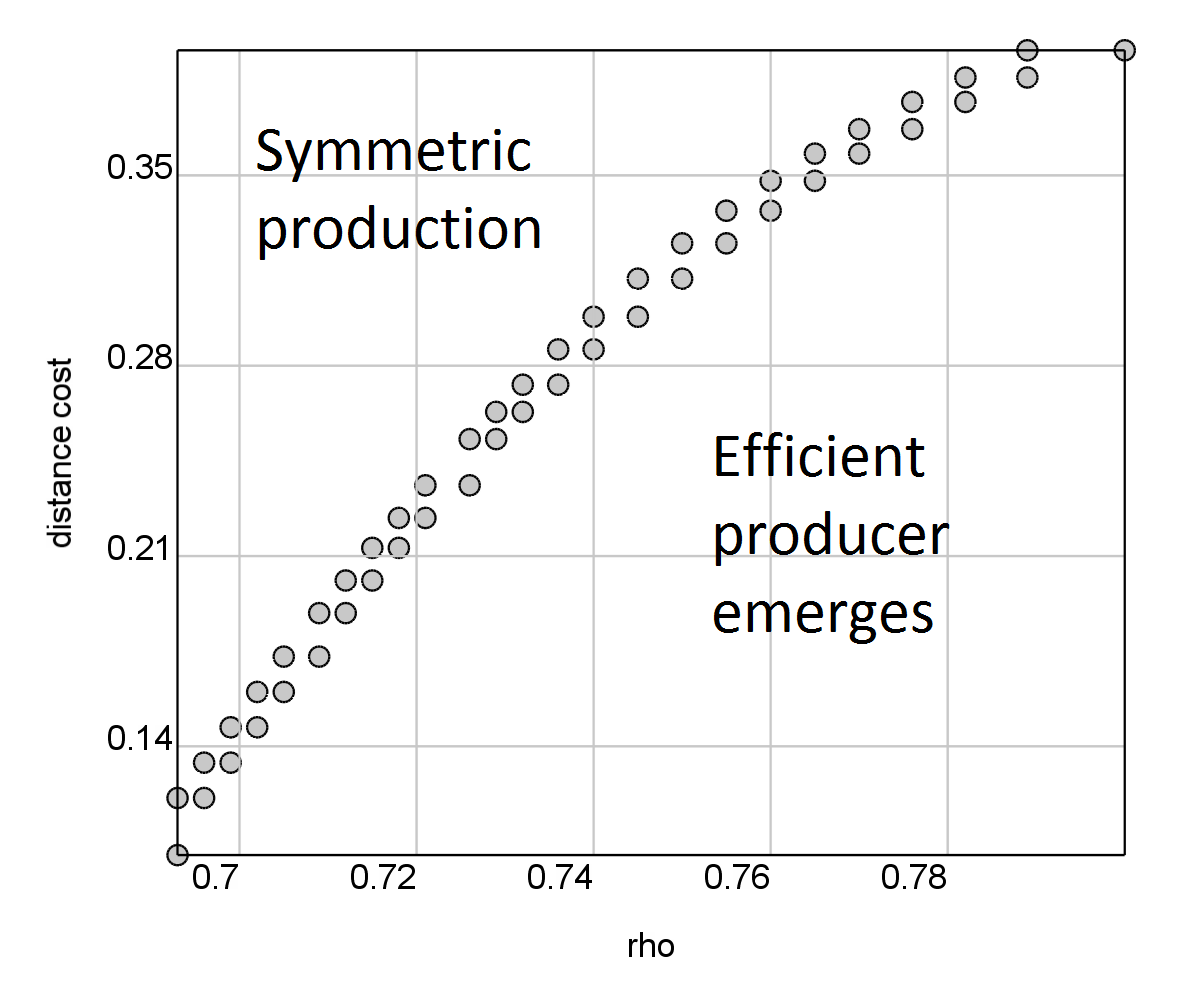
\includegraphics[width=0.8\textwidth]{ChapterConnectedModels/Figures/HG_modelday_96878_TwoRegionTransmission_Mon-May-20-08_37_46-BST-2013__rho_vs_deliveryCostwText}}
\caption{Two region transmission belt model: one Person, one Firm per region, starting off in symmetric production. $\rho$ and distance costs start low. Each is raised in turn. When an efficient producer dominates through economies of scale as one is raised, the model shifts to raise the other until equilibrium moves back to symmetry again. A data point is taken at each shift as the parameter sweep threads through equilibria. \label{fig:paramSweepLoVDelCost}}%
\end{figure}

Figure \ref{fig:paramSweepLoVDelCost} presents a series of data points where the transmission belt model moves between production equilibria. The process for creating this graph was as follows. Distance costs begin at $0.1$ and $\rho$ at $0.1$. At these values, the model is in a symmetric equilibrium as described in section \ref{sec:lov_vs_eos} and lowering those values further does not alter that state. Rather than just sample points in the parameter space, a thread is woven back and forth across the equilibrium transition point, in order to demonstrate that the model is moving between production regimes. Each variable takes a turn to increase slowly, in increments of $0.001$ spaced apart by a gap of three hundred days to let any change settle down, starting with $\rho$. The model tips over out of symmetry when goods become substitutable enough for efficiency of production to win over \gls{lov}. At this transition point, the model is made to pause again for a set number of days to allow oscillations to dampen. Distance costs between the two regions are then increased until gains from efficiency are lost and the model reverts back to the symmetric equilibrium. The two variables are alternately threaded across the transition point in this way to map the line along which the equilibria are divided.

%Explaining why lock-in occurs if people are allowed to move. I can't currently think of any interesting way to show this graphically. 
In the above example, when one Firm becomes the more efficient producer, utility is higher for the Person in their region: they face no distance costs to buy from the cheapest, most efficient source and thus have an advantage over the more distant Person. In the \gls{coremodel} this difference in utility would be an indication that agents want to move to the better region. In the transmission belt model, if People are allowed to move, this does happen - but the result is different to the core model, in that once People have moved to the more efficient region, this outcome is `locked in'. If People have chosen one optimal region, the amount of time input they bring with them locks the Firm in their region into efficient production. This is not quite a complete `black hole' outcome as, in the transmission belt model, Firms are not making separate location decisions and so one remains in the now-deserted region, and receives demand. But it is a black hole for the People: there is no incentive for them to leave the region they have moved to.
 
Note that providing a permanent level of fixed demand in both regions (as the \gls{coremodel} does with its agricultural sector) makes no difference to this dynamic. In the \gls{coremodel}, this fixed demand provides a path between equilibria where people and firms can migrate in both directions; the symmetric outcome can be a stable equilibrium at high distance costs. The transmission belt model, however, only requires a single Person out of many to be mobile for `lock-in' to occur in the more efficient region.

\subsubsection{Two Firms per region \label{sec:twofirmsperregion}}
%Two Firms in each region
\begin{figure}[p]
\centering
\subfloat[$\rho= 0.5$, distance cost $=0.1$]{\label{fig:fourFirmSymmetry}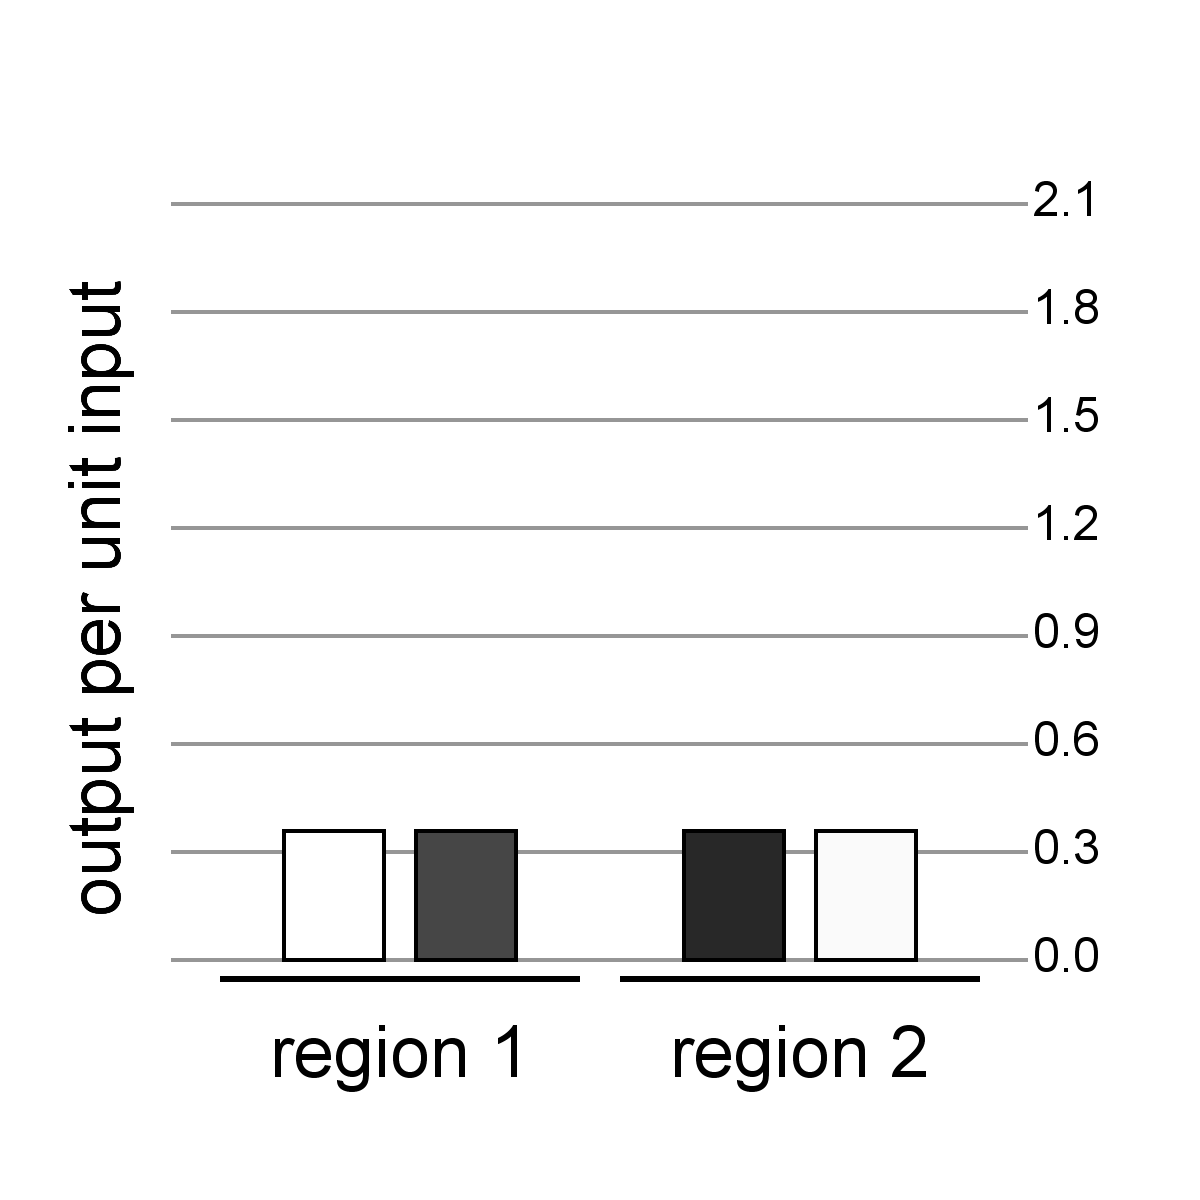
\includegraphics[width=0.49\textwidth]{ChapterConnectedModels/Figures/JS_modelday_5066_TwoRegionTransmission_Wed-May-22-15_50_12-BST-2013__MainViz}}
\hspace{0.1}
\subfloat[$\rho= 0.77$, distance cost $=0.1$]{\label{fig:fourFirmOneEff}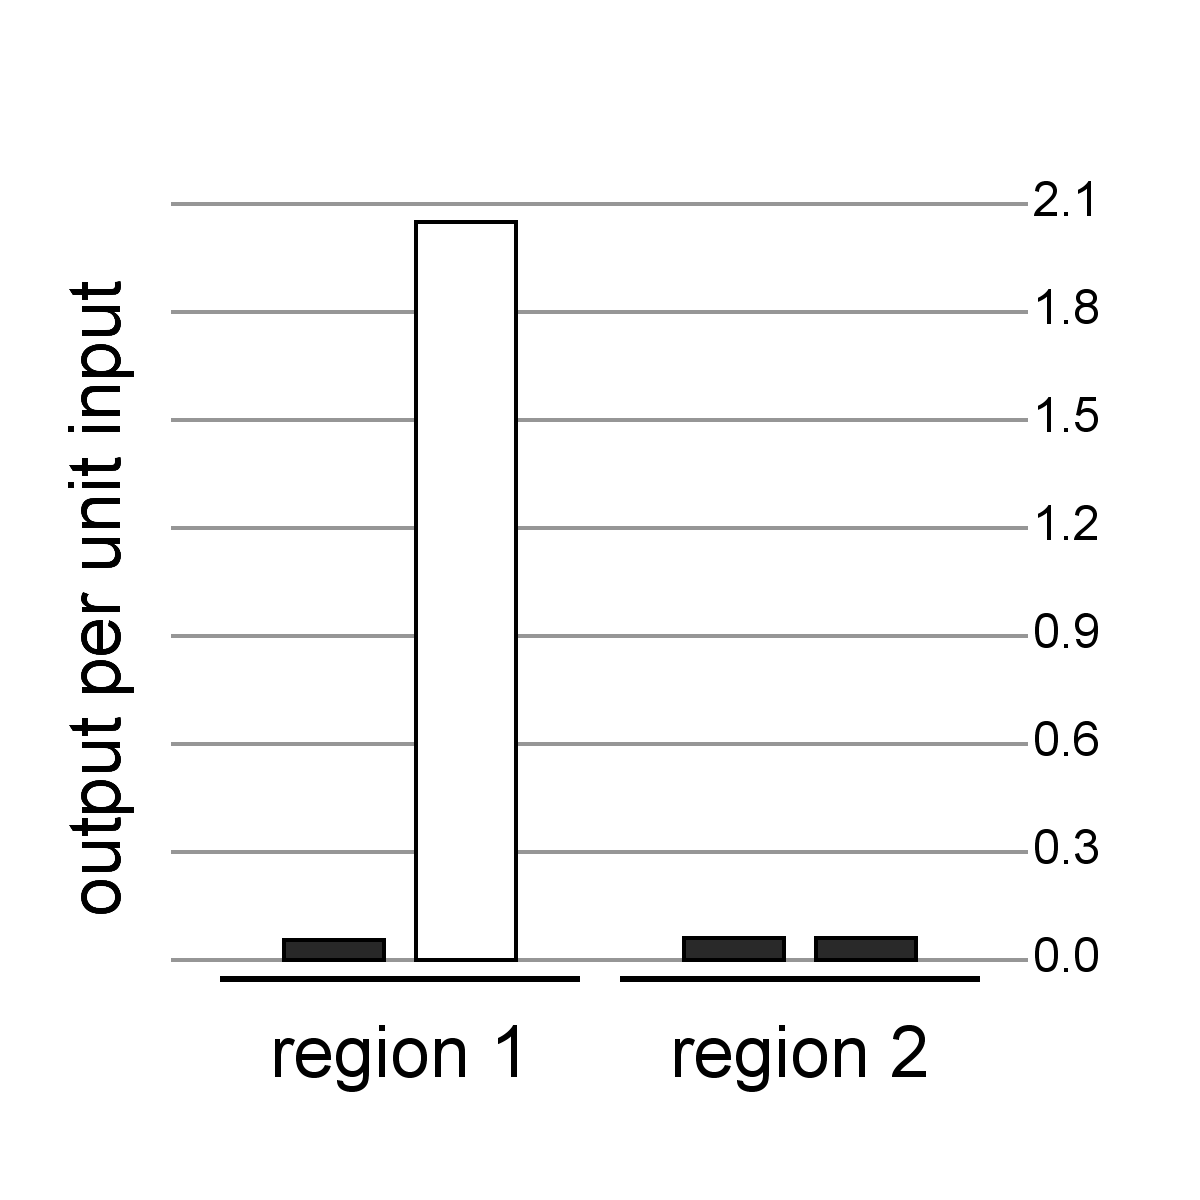
\includegraphics[width=0.49\textwidth]{ChapterConnectedModels/Figures/JT_modelday_7931_TwoRegionTransmission_Wed-May-22-15_50_34-BST-2013__MainViz}}
\hspace{0.1}
\subfloat[$\rho= 0.77$, distance cost $=0.35$]{\label{fig:fourFirmMix}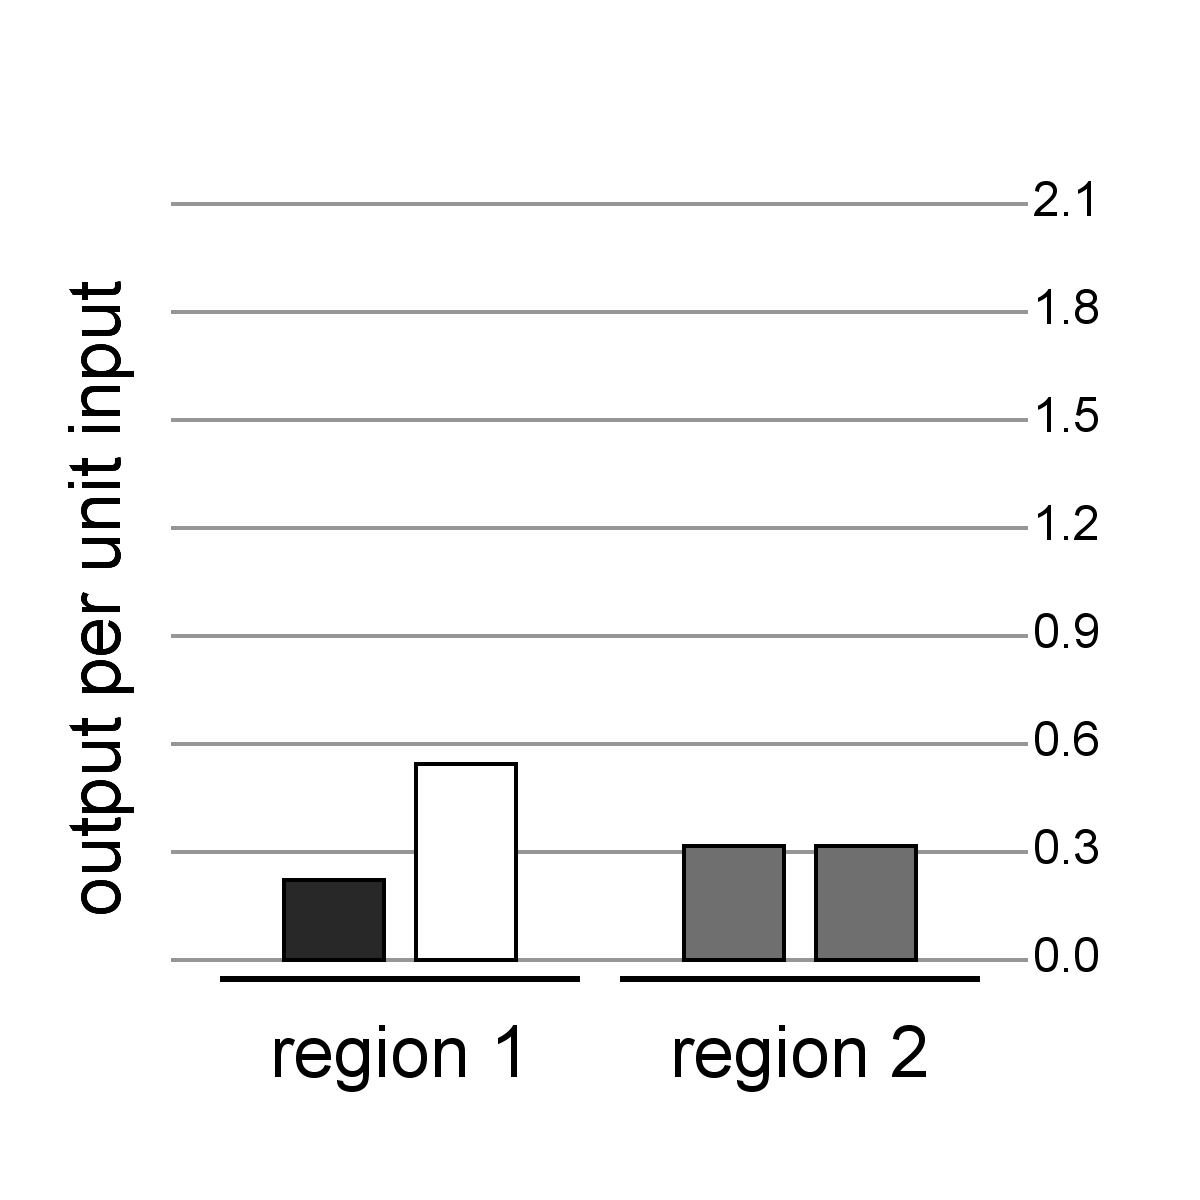
\includegraphics[width=0.49\textwidth]{ChapterConnectedModels/Figures/JU_modelday_12623_TwoRegionTransmission_Wed-May-22-15_51_11-BST-2013__MainViz}}
\hspace{0.1}
\subfloat[$\rho= 0.85$, distance cost $=0.55$]{\label{fig:fourFirmTwoEff}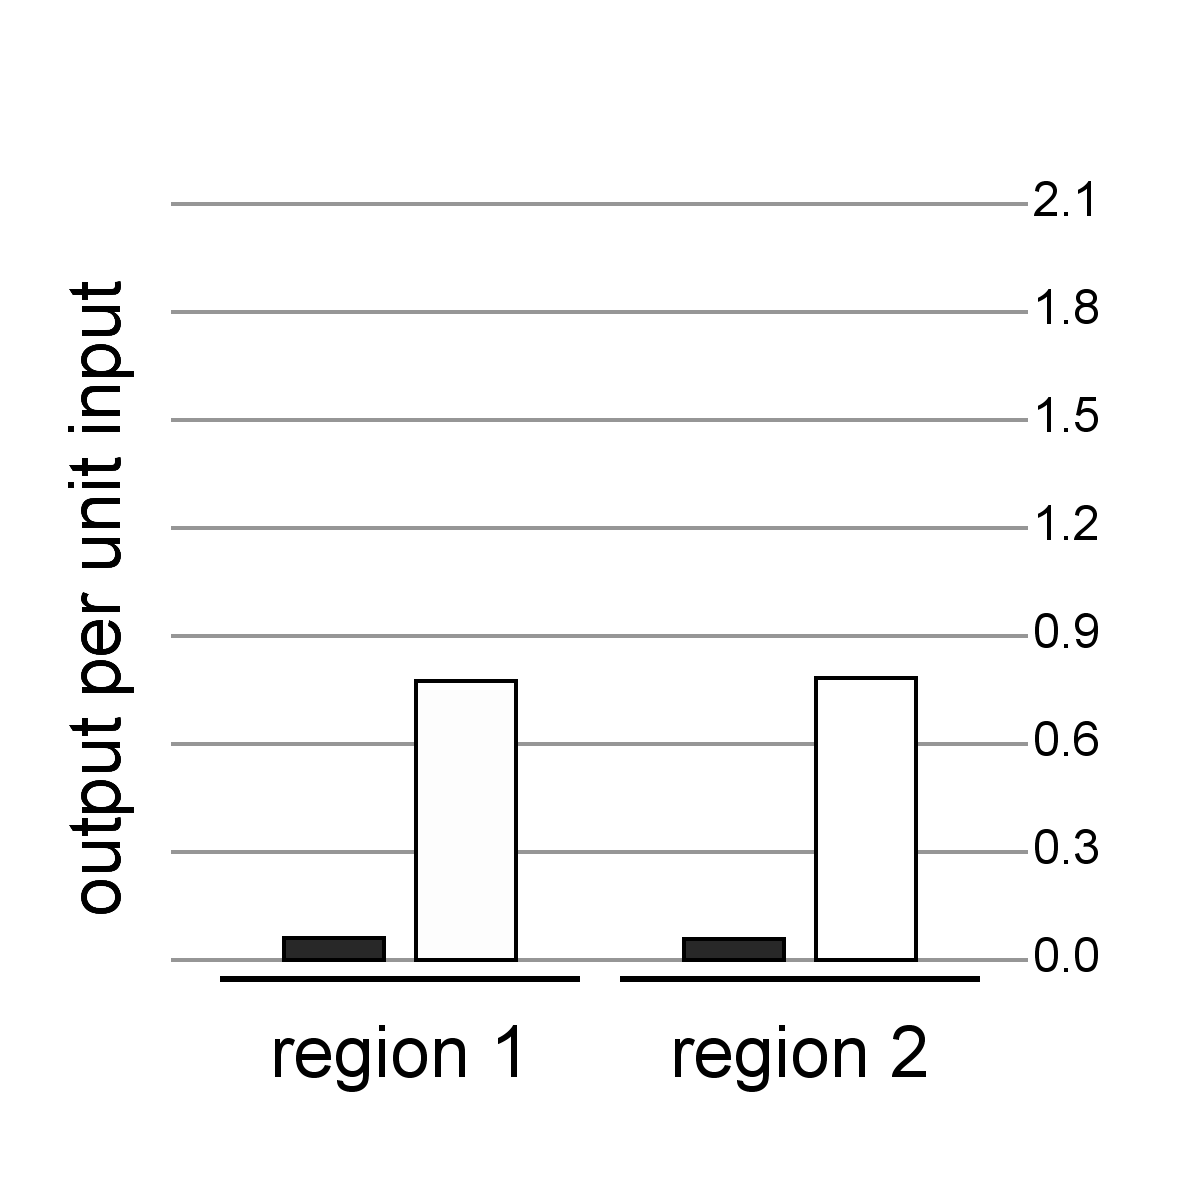
\includegraphics[width=0.49\textwidth]{ChapterConnectedModels/Figures/JV_modelday_17290_TwoRegionTransmission_Wed-May-22-15_51_49-BST-2013__MainViz}}
\caption{Two regions, two Firms in each region. Varying $\rho$ and distance costs determines production regime, which can vary within each region. Y-axis shows output per unit input: higher values indicate more efficient production scale. \label{fig:FourFirmTwoRegion}}%
\end{figure}
%Two Firms per region, with two People static again, one per region. Four different kinds of production regime are possible by varying $\rho$ and distance cost, demonstrating heterogeneity within regions as well as between them.

Adding a second Firm to each region (taking the model total to four) reveals another dynamic resulting from the interaction of \gls{lov}, \gls{eos} and distance. The internal production structure of each region can vary, as well as the production regime of the whole model. Figure \ref{fig:FourFirmTwoRegion} shows the efficiency of the two firms each Region, in terms of `output per unit input'. The higher this is, the more efficiently the Firm is producing, due to having more time input from People buying its good. (The \gls{eos} curve and magnitude parameters are both set to $0.5$ as this keeps the model stable when two People are buying.) The firms are shaded white to dark grey, where white is the highest efficiency and dark grey the lowest. 

Figure \ref{fig:FourFirmTwoRegion} shows the four states the model takes at differing values of $\rho$ and distance cost. At the lowest values, when \gls{lov} is high and distance costs low, production spreads evenly across the model. A large proportion of People's time is lost to distance, but this is outweighed by the utility gains from a higher \gls{lov}. As \gls{lov} decreases, a single more-effficient producer emerges. This is possible due to lower distance costs; as these are increased, the regime changes again through two more states. In sub-figure \ref{fig:fourFirmMix}, the regions diverge: one reverts to its own internal symmetry while the other splits between more and less efficient producers. In the final sub-figure, as distance costs become higher and goods more substitutable, a more-efficient producer emerges in each region. This contrasts to the \gls{coremodel}: regions can develop internal structure, and this development between and within regions is dependent on model-wide interaction.

\subsection{Space and welfare outcomes in a many-agent model \label{sec:spacenwelfare}}

\begin{figure}[p]
\centering
\subfloat[Demand spread out: $\rho= 0.7$, distance cost $=4.75$. Firm y-axis scale to $0.4$. For People, double line marks utility mean.]{\label{fig:lineModelSpreadOut}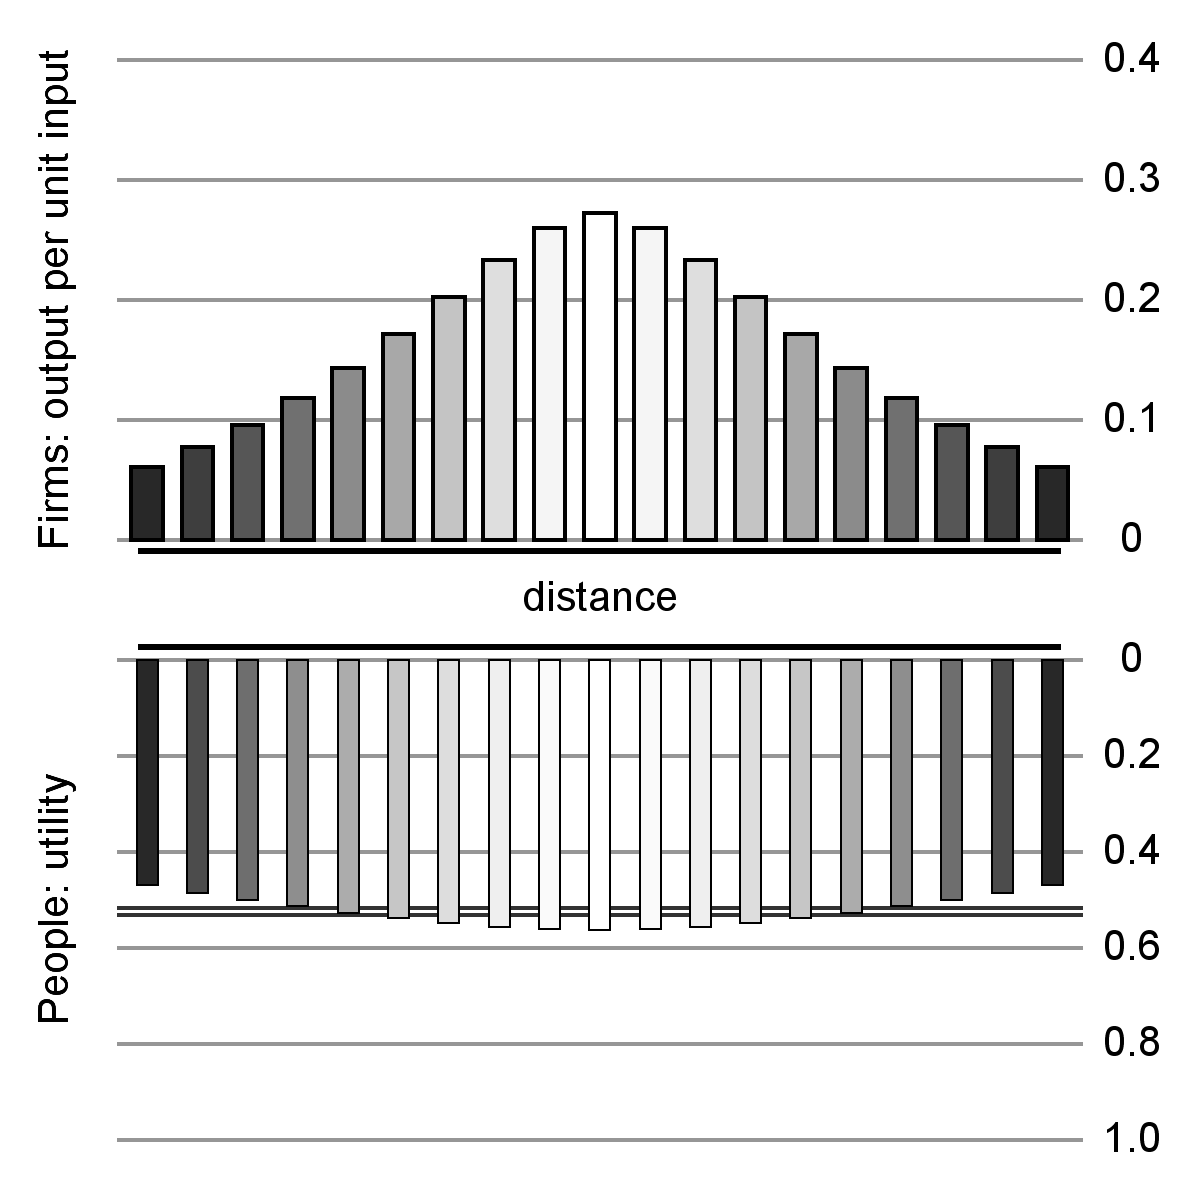
\includegraphics[width=0.6\textwidth]{ChapterConnectedModels/Figures/JY_modelday_948_1DLineManyAgentsTransmission_Wed-May-22-16_09_15-BST-2013__MainViz}}
\hspace{0.1}
\subfloat[Efficient producer emerges: $\rho= 0.7$, distance cost $=4.5$. Firm y-axis scale to $3.1$, with $0.4$ marked for comparison.]{\label{fig:lineModelOneEff}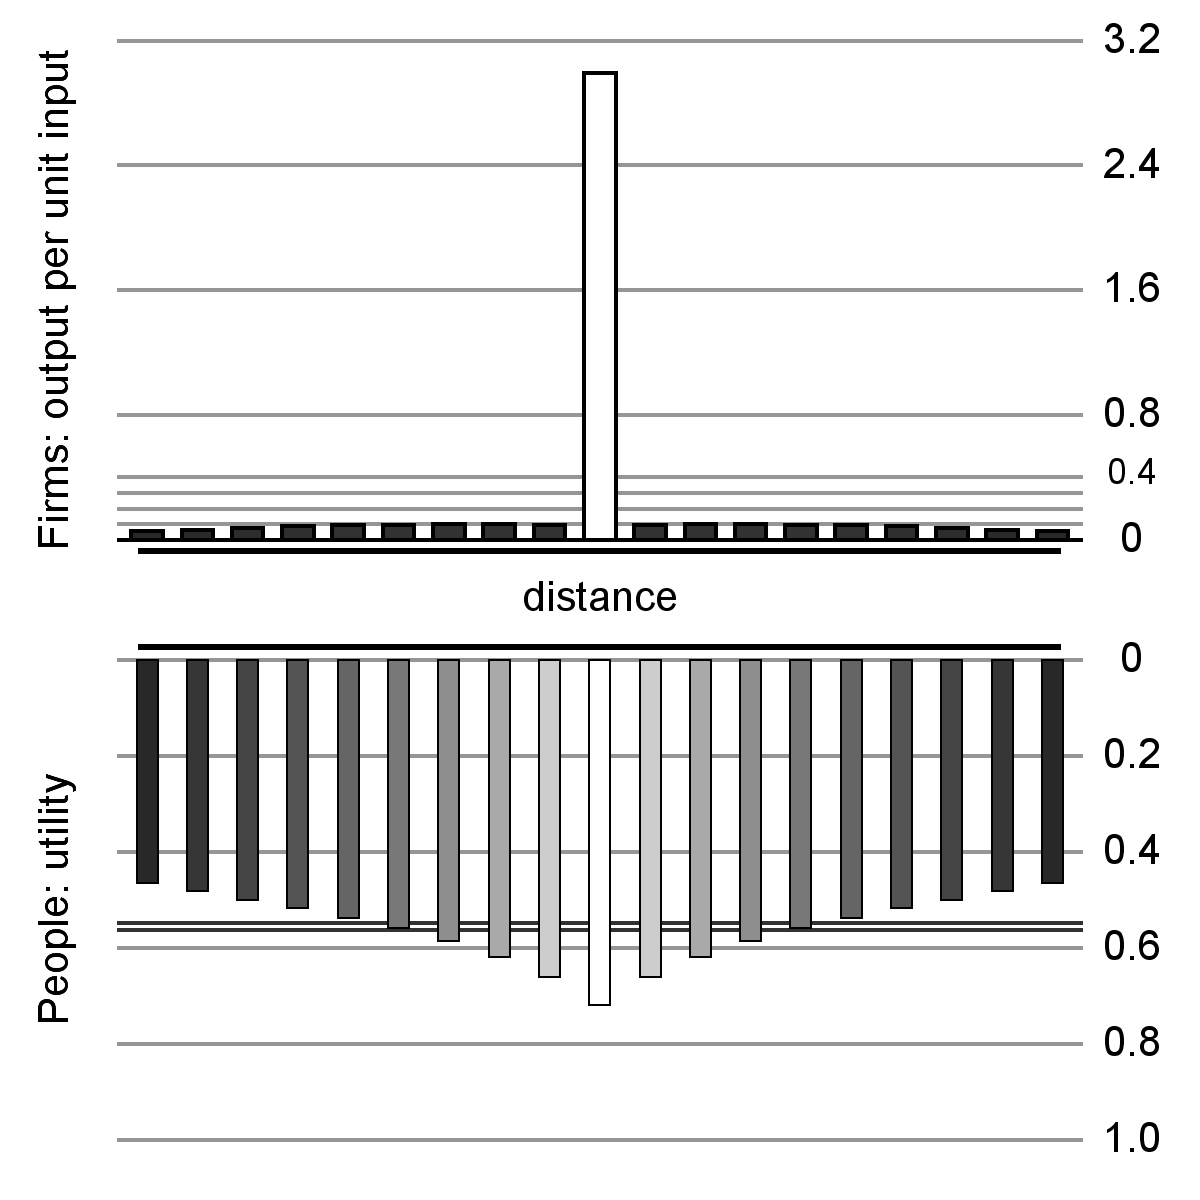
\includegraphics[width=0.6\textwidth]{ChapterConnectedModels/Figures/JW_modelday_1051_1DLineManyAgentsTransmission_Wed-May-22-16_06_33-BST-2013__MainViz}}
\caption{$19$ People, $19$ Firms, spaced between $0$ and $1$ on a line. Distance cost determines transition between production regimes. Double black line across People's utility marks the mean utility value. Different scales used for Firm efficiency y-axis; the second figure marks the lower values used in the first. \label{fig:lineAgentsTransmissionBelt}}%
\end{figure}

\begin{figure}[p]
\centering
\subfloat[Two more-efficient producers: $\rho= 0.73$, distance cost $=8.5$. Firm y-axis scale to $2$.]{\label{fig:lineModelTwoFirms}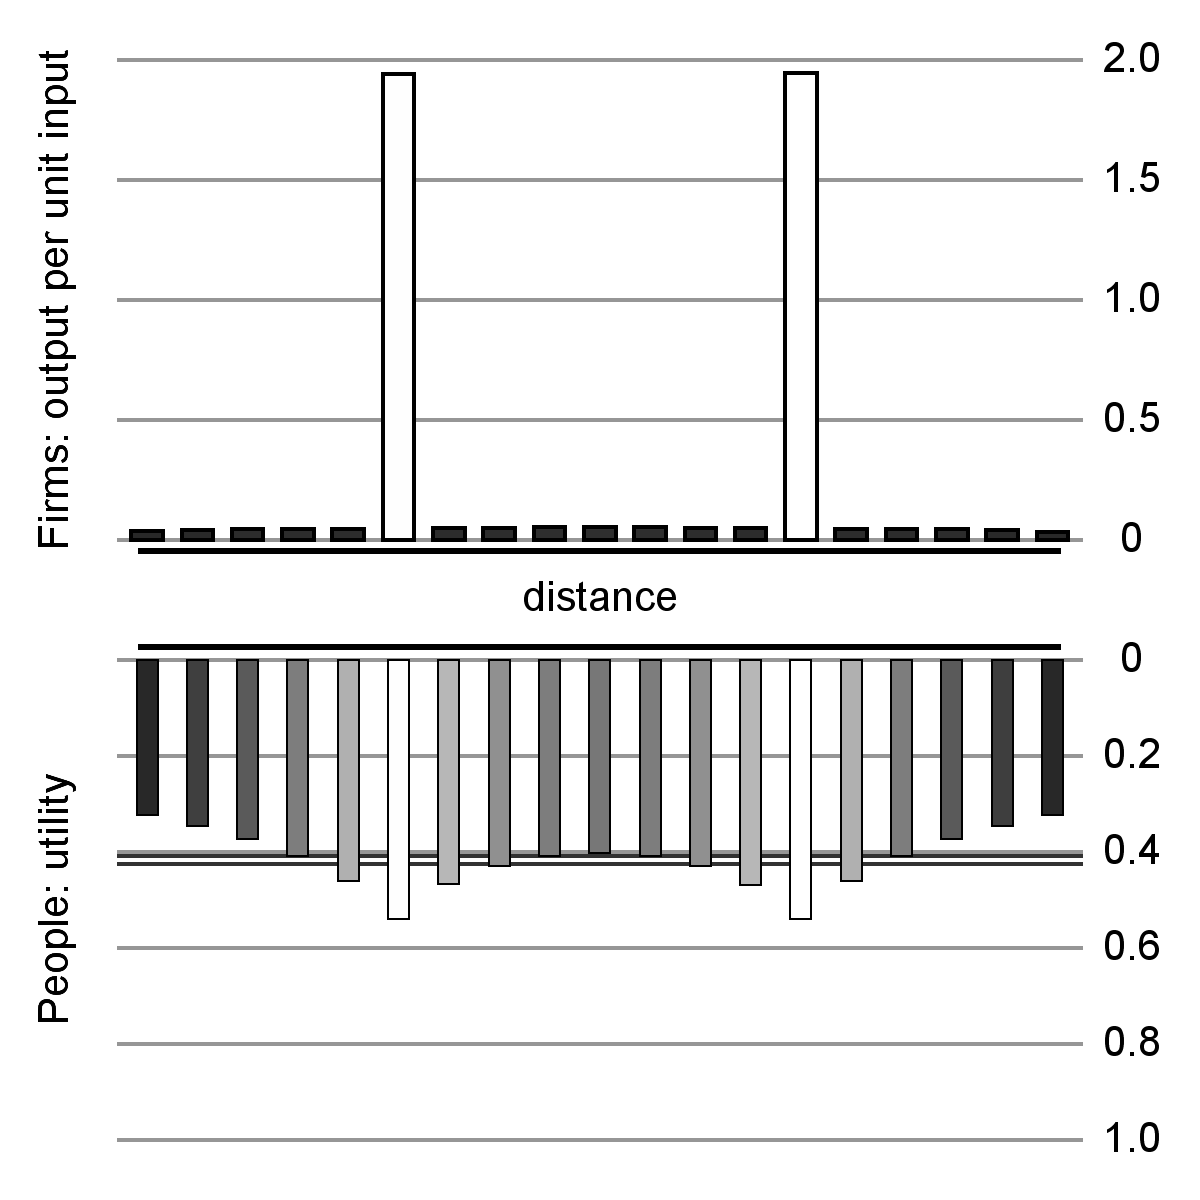
\includegraphics[width=0.6\textwidth]{ChapterConnectedModels/Figures/JZ_modelday_1333_1DLineManyAgentsTransmission_Wed-May-22-16_12_29-BST-2013__MainViz}}
\hspace{0.1}
\subfloat[Many more-efficient producers emerge: $\rho= 0.79$, distance cost $=45.5$. Firm y-axis scale to $0.4$]{\label{fig:lineModelManyFirms}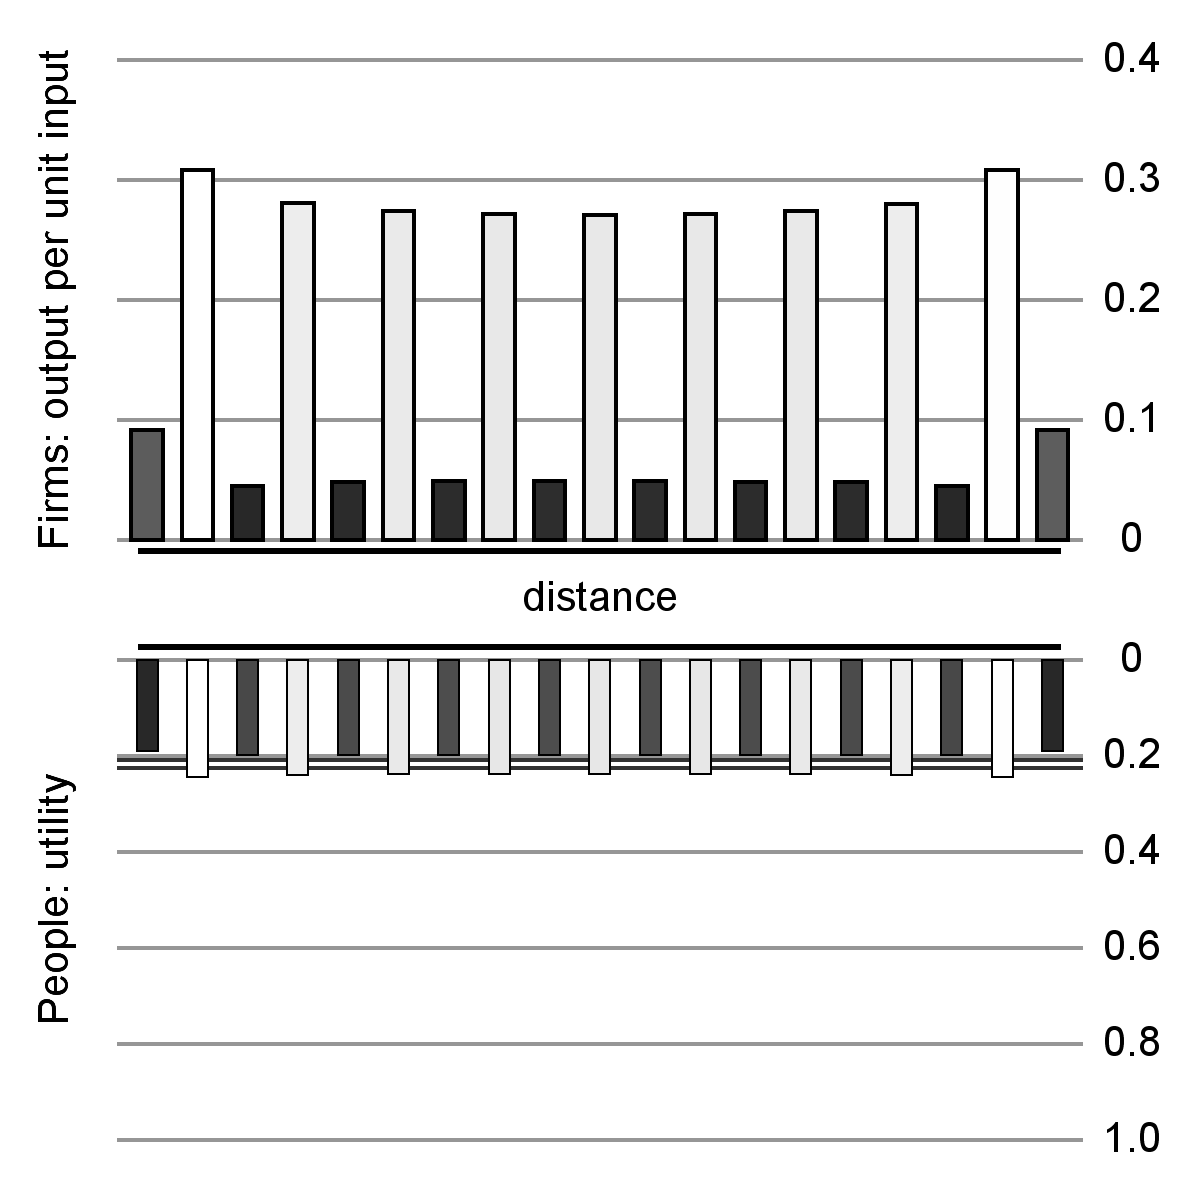
\includegraphics[width=0.6\textwidth]{ChapterConnectedModels/Figures/KA_modelday_1423_1DLineManyAgentsTransmission_Wed-May-22-16_14_52-BST-2013__MainViz}}
\caption{$19$ People, $19$ Firms, spaced between $0$ and $1$ on a line. Two examples of different more-efficient production regimes emerging for differing values of $\rho$ and distance cost. \label{fig:lineAgentsTransmissionBelt2}}%
\end{figure}

Increasing the transmission model's number of agents produces similar dynamics as in the previous section. In this section's example,  a larger number of Firms and People interact to produce equilibrium outcomes. Nineteen Firms and Nineteen people have evenly spaced locations along a line of distance $1$; every location containing a Firm also contains a Person. An odd number is chosen so that one Firm/Person pair is directly in the centre of the line. With many agents on a line, the transmission model is very sensitive to parameter settings: many combinations lead to the kind of positive feedback described in section \ref{sec:markup}. This section selects sets of parameter values able to maintain stability between production regime changes.
%\cmt{Remember: EoSC = 0.1, EoSM = 0.1. In the two-region, they're 0.5. Explain why. (needed to explain y axis vals.}
%Ah OK: I think I see what I was saying / saw - increasing delivery costs once the efficient producer has emerged is obviously detrimental to those further away. In the core model, this kind of tension between utility levels is not possible: it's the driver for mobility. Here - without a specific disutility from being at a particular place - mobility just leads to the `black hole' outcome.

Figure \ref{fig:lineAgentsTransmissionBelt} shows these pairs of $19$ People and Firms with distance represented on the horizontal axis. Above the `distance' line, each Firms' efficiency levels are shown: their output per unit input. Below the `distance' line, each Person's utility level is shown. A double line marks the mean utility for all People. White-to-dark colouring marks the relative spread of high to low values for the iteration on which the graph was produced. Sub-figure \ref{fig:lineModelSpreadOut} shows symmetric production - no more-efficient producers have emerged. Those nearest the centre of the line have the highest utility and the highest input of time. People closer to the centre are better off simply due to being closer to a wider range of Firms. Those nearer to edge can access less quantity of nearby goods. Equally, the central Firm gets the most input due to its position. 

In sub-figure \ref{fig:lineAgentsTransmissionBelt}, distance cost has been reduced from $4.75$ to $4.5$, resulting in the central Firm emerging as an efficient producer. Note the difference in scales for Firm efficiency: the bottom sub-figure marks the value of $0.4$, which is the maximum for the top. The efficiency gain is large.

Figure \ref{fig:lineAgentsTransmissionBelt2} shows two results where more-efficient production regimes have emerged. By increasing distance costs in each case, they illustrate that it can determine the specific equilibrium production morphology. These are each pushed up the same path of distance cost and \gls{lov} outlined in section \ref{sec:TM_space}. In this case, positions further up the distance cost / \gls{lov} curve produce a larger number of efficient producers. 

Transitions to more efficient production \emph{never} make any single Person worse off. It is trivially true that, if People's locations are fixed, increasing distance costs will make those further away from the more-efficient producers worse off than others able to minimise those costs. But the transitions to more efficient production regimes always produce both higher aggregate welfare at the same time as making each individual better off, or at the very least, no Person worse off. To the extent that larger demand from more proximate People is responsible for tipping the transmission belt model over into more efficient production, this is a positive externality for others able to benefit from cheaper goods produced at the larger scale.

\subsection{Combining the transmission belt model with density cost \label{sec:tbmplusdensity}}
\begin{figure}[]
\centering
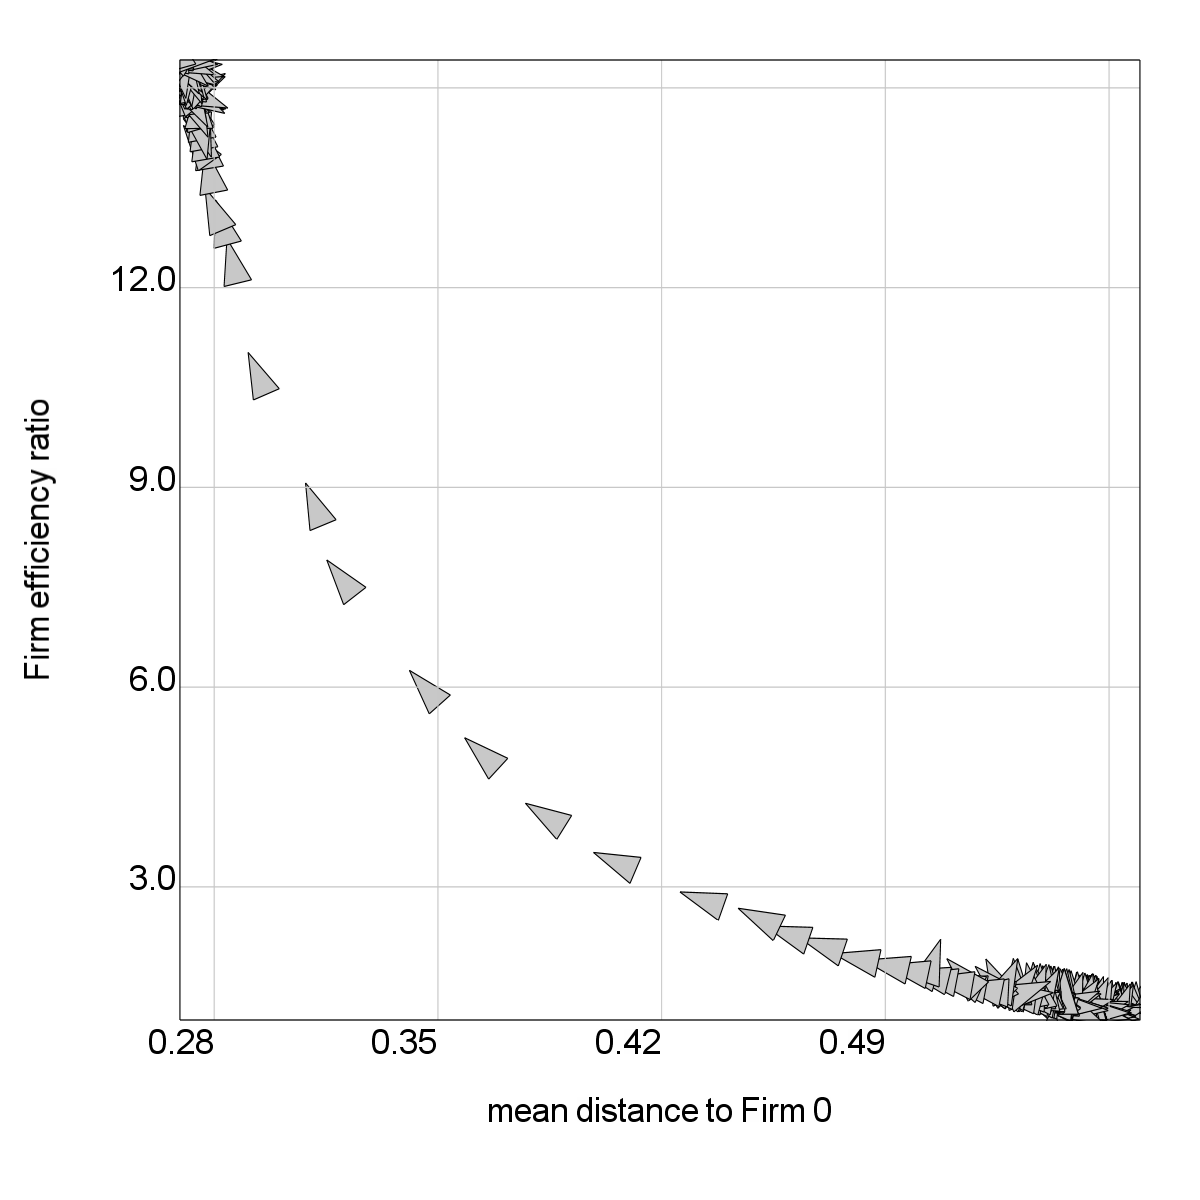
\includegraphics[width=0.9\textwidth]{ChapterConnectedModels/Figures/VK_modelday_993_TransmissionPlusDensity1_Sat-Jun-08-16_33_48-BST-2013__distanceToCentralFirm_vs_productionLeveledit}}%
\caption{Two Firms fixed a distance of $1$ apart; a more-efficient producer emerges as $\rho \rightarrow 0.9$. Mean distance to Firm $0$ (thus mean distance from Firm $1$) vs Firm production ratio; arrows point in direction of change between model iterations.  \label{fig:TransmissionDensity2}}%
\end{figure}

\begin{figure}[]
\centering
\subfloat[$R^2$ space visualisation, $\rho=0.5$]{\label{fig:LoVlow2}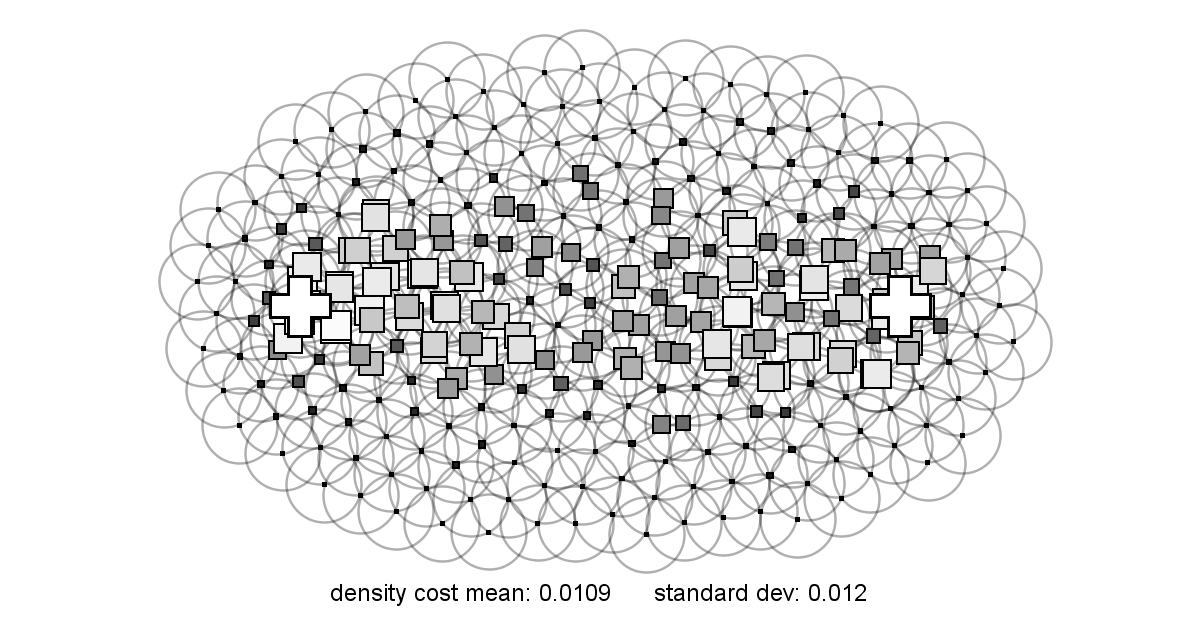
\includegraphics[width=1\textwidth]{ChapterConnectedModels/Figures/TBDensity1a}}%
\hspace{0.1}  
\subfloat[$R^2$ space visualisation, $\rho=0.9$]{\label{fig:LoVhigh2}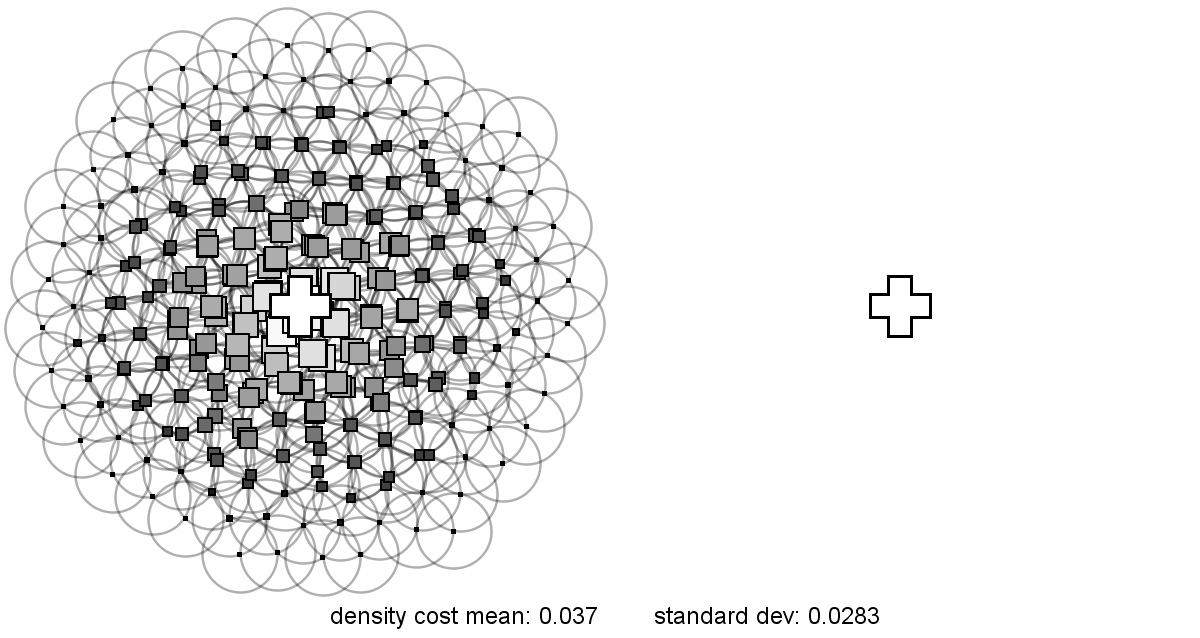
\includegraphics[width=1\textwidth]{ChapterConnectedModels/Figures/TBDensity2a}}%
\caption{Two Firms fixed a distance of $1$ apart; a more-efficient producer emerges as $\rho \rightarrow 0.9$. \label{fig:TransmissionDensity}}%
\end{figure}

The final result presented in this section builds on the two-Firm \gls{lov} example presented in section \ref{sec:LoVresult}. In that scenario, two Firms at fixed positions in an $R^2$ space were given exogenously fixed distance costs, with one Firm having double the distance cost of the other. The aim was to show the effect of changing \gls{lov} in this scenario and how it interacted with density cost: as \gls{lov} increases, it is more valuable to be closer to the more expensive good and `buy the other in' from further away. 

%By fully linking supply and demand with the transmission belt model, this section can endogenise the outcome. 
This example demonstrates that a fully linked supply/demand model is able to endogenise something  - in this case, the particular region that emerges as the `core' - that previously had to be exogenously imposed. There are no initial differences between the Firms. Some parameters are set differently to section \ref{sec:LoVresult} to allow the model within the correct range for transitioning between production equilibria. Distance costs are $0.25$ and the number of People is $300$. The \gls{eos} curve parameter is set to $0.001$ to stop Firms from `tipping over' as those $300$ people send demand signals every time step. Otherwise, the outcome as regards which region emerges as the more-efficient is down to chance. This section illustrates the result for Firm 0 becoming the more-efficient producer.

As $\rho$ is increased (and \gls{lov} drops), more-efficient production starts to kick in - producing a cheaper good. Figure \ref{fig:TransmissionDensity2} shows this transition as $\rho$ moves from $0.5$ through to $0.9$. As in section \ref{sec:LoVresult}, the x axis shows the mean distance to Firm $0$ (and thus, because there are only two firms, this is the inverse of the mean distance from Firm 1). The y axis is the ratio between production efficiency for the two Firms, always placing the higher-efficiency Firm in the numerator, thus making sure the ratio is $ \geqslant 1$. 

This correlation graph introduces a different way to view model time: arrows point in the direction that values changed between iterations. A vector is found between $t-1$ and $t$ and its angle used. The transition to a single more-efficient firm is thus clearly visible: the arrows indicate mean distance to Firm $0$ dropping as the Firm efficiency ratio climbs to $~13$. Visualisations of the agents in this $R^2$ space are given in figure \ref{fig:TransmissionDensity} for the two values of $\rho$, each side of the transition. People's squares indicate, in this case, the relative range of incurred density cost. As the higher-efficiency producer emerges, they move nearer to that production sight. As this is also in the same direction of travel indicated by section \ref{sec:LoVresult} as \gls{lov} drops, the result is doubly locked in.

%Section \ref{sec:TM_space} noted that, if People are allowed free movement in a discrete two-region version of the transmission belt model, they will all move to a single region and buy in from the distant Firm. 
%Want to start by saying this is example of mutual exclusivity really; not a great deal of analytic use combining density etc. Slightly `soporific' quality etc. 
%The density cost approach from section x could provide such a disutility, but where in that section it had a rationale, in this context it is much more like one of Krugman's `soporific qualities': People will move away because staying is not good, but only because an imposed cost of being here \emph{makes} it so. 
\section{Summary \label{sec:tbconc}}

This chapter has introduced an agent-based spatial economic model linking supply and demand to produce a `general' spatial equilibrium able to transition between production equilibria while allowing agents heterogenous locations. It could be argued the model has four key `general' components out of a possible five. One: the demand side works effectively, allowing People to make separate optimal buying choices that account for location and \gls{lov}. Two: the supply side has a functioning production system, able to turn that demand into an equilibriating, stable economy that can shift between production regimes as key parameters change. Three: firms are able to gain a profit from the market. Four: it has an effective price system able to tie these separate components together into a `general' whole. What it lacks is a fifth key element: competition between Firms.

Section \ref{sec:markup} demonstrated that it is possible for Firms to gain a `profit' and that doing so has external effects on other Firms (as well as People). However, it does not find a way to create a competitive market structure through emergent Firm interaction. The specific route the transmission belt model found to achieving a `general' model appears to make this kind of competitive dynamic challenging. In comparison, the \gls{coremodel} contains a detailed argument about market structure and competition. The \gls{dxs} approach it is built on is a careful web of reasoning that attempts to deal with competition effects in an increasing returns setting. It is difficult to directly compare approaches on this point, as the market structure of the \gls{coremodel} involves assuming equilibrium has been reached. 

Nevertheless, the transmission belt model presented in this chapter has some advantages. It is very much in the \gls{abm} tradition of examining the \emph{process} of moving between equilibria. The ability to transition between production equilibria is something the \gls{dxs} approach rules out. All goods are assumed to be produced symmetrically, at the same scale. Increasing returns are still present but, as section \ref{sec:coremodel} explained, a series of stages transform production-level \gls{eos} into a change in firm number and thus in utility levels via \gls{lov}. 

More fundamentally, the model's equilibrium states come about with no central directing mechanism. This happens entirely through a distributed spatial price interaction between individual Firms with \gls{eos} and individual People's demand for goods. It can allow for those agents to have heterogenous locations and for People to optimise those locations. 

This comparison to \gls{ge} is taken up further in the conclusion. 










